%% }
%% Copyright 2007-2020 Elsevier Ltd
%% 
%% This file is part of the 'Elsarticle Bundle'.
%% ---------------------------------------------
%% 
%% It may be distributed under the conditions of the LaTeX Project Public
%% License, either version 1.2 of this license or (at your option) any
%% later version.  The latest version of this license is in
%%    http://www.latex-project.org/lppl.txt
%% and version 1.2 or later is part of all distributions of LaTeX
%% version 1999/12/01 or later.
%% 
%% The list of all files belonging to the 'Elsarticle Bundle' is
%% given in the file `manifest.txt'.
%% 

%% Template article for Elsevier's document class `elsarticle'
%% with numbered style bibliographic references
%% SP 2008/03/01
%%
%% 
%%
%% $Id: elsarticle-template-num.tex 190 2020-11-23 11:12:32Z rishi $
%%
%%
%\documentclass[preprint,12pt]{elsarticle}
\documentclass[preprint,10pt]{elsarticle} % lancet: text font 10 
%\documentclass[review,10pt]{elsarticle} % lancet: text font 10 
\usepackage{float}
\usepackage{amsmath}
\usepackage{graphicx}
%\usepackage[unicode=true, bookmarks=false]{hyperref}
%\usepackage[latin9]{inputenc}
\usepackage{times} % lancet: times new roman
\usepackage[verbose,tmargin=1in,bmargin=1in,lmargin=1in,rmargin=1in]{geometry}
\usepackage{setspace} 
\singlespacing % lancet: single spacing
\usepackage{lineno}
\modulolinenumbers[5]
%\linenumbers


%% Use the option review to obtain double line spacing
%% \documentclass[authoryear,preprint,review,12pt]{elsarticle}

%% Use the options 1p,twocolumn; 3p; 3p,twocolumn; 5p; or 5p,twocolumn
%% for a journal layout:
%% \documentclass[final,1p,times]{elsarticle}
%% \documentclass[final,1p,times,twocolumn]{elsarticle}
%% \documentclass[final,3p,times]{elsarticle}
%% \documentclass[final,3p,times,twocolumn]{elsarticle}
%% \documentclass[final,5p,times]{elsarticle}
%% \documentclass[final,5p,times,twocolumn]{elsarticle}

%% For including figures, graphicx.sty has been loaded in
%% elsarticle.cls. If you prefer to use the old commands
%% please give \usepackage{epsfig}

%% The amssymb package provides various useful mathematical symbols
\usepackage{amssymb}
%% The amsthm package provides extended theorem environments
%% \usepackage{amsthm}

%% The lineno packages adds line numbers. Start line numbering with
%% \begin{linenumbers}, end it with \end{linenumbers}. Or switch it on
%% for the whole article with \linenumbers.
%% \usepackage{lineno}
\usepackage{caption}
\usepackage{subcaption}
\usepackage[table,dvipsnames]{xcolor}
\biboptions{sort&compress,super}
\usepackage{color} % for the command \textcolor
\usepackage{soul} % for the command \hl
\usepackage{siunitx}

\usepackage{float}
\floatstyle{boxed}
\newfloat{nonfigure}{tbp}{l0nfig}
\floatname{nonfigure}{Box}

\usepackage{tabularray}
\newcommand{\beginsupplement}{%
        \setcounter{table}{0}
        \renewcommand{\thetable}{S\arabic{table}}%
        \setcounter{figure}{0}
        \renewcommand{\thefigure}{S\arabic{figure}}%
     }

\usepackage{titlesec}
\titleformat*{\section}{\large\bfseries\sffamily}
\titleformat*{\subsection}{\normalsize\bfseries\sffamily}
\titleformat*{\subsubsection}{\small\bfseries\sffamily}
\newcommand{\absdiv}[1]{%
  \par\addvspace{.5\baselineskip}% adjust to suit
  \noindent\textbf{#1}\quad\ignorespaces}
\renewenvironment{abstract}{\global\setbox\absbox=\vbox\bgroup
  \hsize=\textwidth\def\baselinestretch{1}%
  \noindent\unskip\textbf{\large Summary}
  \par\medskip\noindent\unskip\ignorespaces}{\egroup}

%%%%%%%%%%%%%%%%%%%%%%%%%%%%%% User specified LaTeX commands.
%track changes on
\newcommand{\add}[1]{\textcolor{blue}{#1}}
\newcommand{\remove}[1]{\textcolor{red}{\st{#1}}}
%track changes off

\providecommand{\tabularnewline}{\\}

\journal{Lancet Planetary Health}

\begin{document}

\begin{frontmatter}

\title{City designs affect transport mode choice and exposure to health risks during and after a crisis: a global observational study}

\author[melb]{Kerry A. Nice\corref{cor1}\corref{contrib}}
\ead{kerry.nice@unimelb.edu.au}
\author[psychiatry,sun]{Jason Thompson\corref{contrib}}
\author[melb]{Haifeng Zhao}
\author[melb]{Sachith Seneviratne}
\author[RMII]{Belen Zapata-Diomedi}
\author[Belfast,phy]{Leandro Garcia}
\author[Belfast]{Ruth F. Hunter}
\author[wash]{Rodrigo Siqueira Reis}
\author[uill,PPE]{Pedro C. Hallal}
\author[imp,nova,ieps]{Christopher Millett}
\author[Belfast]{Ruoyu Wang}
\author[melb,eng]{Mark Stevenson}
%\author[]{et al.}

\cortext[cor1]{Principal corresponding author}
\cortext[contrib]{Authors contributed equally}
\address[melb]{Transport, Health, and Urban Systems Research Lab, Faculty of Architecture, Building, and Planning, University of Melbourne, VIC, Australia}
\address[eng]{Faculty of Engineering and Information Technology and the Melbourne School of Population and Global Health, University of Melbourne, VIC, Australia}
\address[sun]{Centre for Human Factors and Sociotechnical Systems University of the Sunshine Coast, Queensland, Australia}
\address[psychiatry] {Department of Psychiatry, Faculty of Medicine, Dentistry and Health Sciences, The University of Melbourne, VIC, Australia}
\address[RMII]{Healthy Liveable Cities Lab, Centre for Urban Research, RMIT University, Melbourne, Australia}
\address[Belfast]{Centre for Public Health, Queen’s University Belfast, Institute of Clinical Sciences B, Belfast, Northern Ireland, UK}
\address[wash]{Washington University, St. Louis, Missouri, US}
\address[uill]{Department of Kinesiology and Community Health, University of Illinois Urbana-Champaign}
\address[imp]{Public Health Policy Evaluation Unit, School of Public Health, Imperial College London, London, United Kingdom}
\address[nova]{NOVA National School of Public Health, Public Health Research Centre, Comprehensive Health Research Center (CHRC), NOVA University Lisbon, Lisbon, Portugal}
\address[ieps]{Instituto de Estudos para Políticas de Saúde (IEPS), São Paulo, Brazil}
\address[PPE]{Postgraduate Program in Epidemiology, Federal University of Pelotas, Brazil}
\address[phy]{Physical Activity Epidemiology Group, University of São Paulo, São Paulo, Brazil}


%\begin{keyword}
%% keywords here, in the form: keyword \sep keyword
%% PACS codes here, in the form: \PACS code \sep code
%% MSC codes here, in the form: \MSC code \sep code
%% or \MSC[2008] code \sep code (2000 is the default)
%\end{keyword}

\end{frontmatter}

%% \linenumbers

%% main text

%\section*{Abstract (300 words)}
 \absdiv{\textcolor{OliveGreen}{Background}}
Rapid declines in city mobility saw reductions in exposure to transport-related air pollution and associated health risks during the early stages of the COVID-19 pandemic in 2020 as many cities introduced non-pharmaceutical interventions designed to curb the spread of COVID-19. However, these benefits soon reversed in the pandemic's `Recovery' phase (Sep. 2020 onward), especially in cities whose designs afforded mode-shift away from public and active transport in favour of private motor vehicles. The aim of this paper was to understand the association between global city designs, transport mode choice, and population-level risk exposure during 2020.
 \absdiv{\textcolor{OliveGreen}{Methods}}
Graph networks were used to identify city design types based on road and transport infrastructure in 507 global cities. Comparisons between city types were made on the basis of transportation mode shifts, air pollution levels, and associated health outcomes (i.e., cardiovascular disease, ischemic heart disease, respiratory disease, asthma, and reported COVID-19 cases) throughout 2020. City designs demonstrating sustained reductions in transport-related air pollution associated with reduced risk of acute and chronic disease outcomes were identified.
 \absdiv{\textcolor{OliveGreen}{Findings}}
The mean observed reductions in global NO$_{2}$ and PM$_{2.5}$ levels across observed cities in the early months (mid Feb. 2020 to Apr. 2020) of the COVID-19 pandemic were 5.36\% and 16.19\%, respectively. NO$_{2}$ reductions were estimated to have had a positive impact on population health, equating to an estimated reduction in all-cause mortality of approximately 3\% had the deepest pollution reductions observed in the the `Early-crisis' phase (mid Jan to Feb, 2020 been sustained globally, over the long term. Similarly, it would be expected that reductions in PM$_{2.5}$ levels during this same period would translate into substantial asthma risk reductions of between 19\% and 65\% and all-cause mortality of between 13.2\% and 24.6\%. In the later stages of 2020, city designs (primarily in the Americas and Oceania) that afforded a mode shift away from public transit to private motor vehicles during the pandemic's `Recovery' phase tended to demonstrate the poorest outcomes across all air pollution and health measures, even increasing risk levels above pre-pandemic baselines in some cases. By contrast, cities located in Japan and Korea demonstrated little change in pre- and post crisis transport mode choice, maintaining comparatively low levels of air pollution, associated disease risk, and reduced rates of infectious disease transmission throughout the observation period. Contrasting experiences of road injury in the post-pandemic phase (post 2020) are also observed between these locations.
 \absdiv{\textcolor{OliveGreen}{Interpretation}}
This study illustrates the transient environmental and health benefits observed during the early stages of the COVID-19 pandemic, marked by significant reductions in transport-related air pollution and associated health risks due to imposed non-pharmaceutical public health interventions. City design appears to have played a crucial role in observed pollution and health risk differences between cities, with those that afforded a shift away from public and active transport towards private vehicles witnessing a rapid erosion of pollution-related health benefits gained in the early to mid-phases of the pandemic. These negative effects appear to have also transferred through to rates of road trauma with a resurgence in road injury above pre-pandemic levels, particularly within countries reliant on private motorised transport. Conversely, cities in Japan, South Korea, and select European regions, which did not experience modal shift toward cars sustained reductions in air pollution and have continued a trend of declining road transport injuries. This underscores city design as a significant factor in navigating pandemic-related challenges and suggests city designs containing higher levels of public and mass transit appear to demonstrate greater levels of resilience in the face of infectious disease threats. 
 \absdiv{\textcolor{OliveGreen}{Funding}}
 KAN, JT, and SS are supported by NHMRC 2019/GNT1194959. JT is supported by ARC FT220100650. CM is supported by the NIHR GHRC on NCDs and Environmental Change (NIHR203247) using UK aid from the UK Government to support global health research. RFH is supported by funding from the UKPRP and ESRC (grant refs MR/V049704/1 and ES/V016075/1.


\fbox{\parbox{\textwidth}{
    \subsection*{\textcolor{OliveGreen}{Research in context}}
    \subsubsection*{Evidence before this study}
       Previous studies have highlighted reductions in transport and industrial-related air pollution and associated health risks for select locations during 2020, linked to reductions in city mobility during the COVID-19 pandemic. Studies have also observed subsequent resurgence in air pollution and road collision risk for select cities and locations in the post-pandemic phase. 
    \subsubsection*{Added value of this study}
       This study adds a global perspective by analysing changes in health risks associated with levels of air pollution during 2020 across 507 cities and linking that to previously established city design types. By including such a large sample of locations, it enables comparison between city types and demonstrates how differences in the initial reduction and then resurgence of air pollution and associated health risks over the course of 2020 were associated with urban design characteristics.
    \subsubsection*{Implications of all the available evidence}
    Our results indicate that city designs that enable adaptation to crises through rapid transition from public/active transport modes to private transport may ultimately endure worse public health outcomes across a syndemic of chronic disease, infectious disease, and road injury if these patterns of behaviour become entrenched. Cities that offered a  diversity of public, active, and private transport options and did not trade off public transport ridership for private transport, demonstrated greater resilience in the face of the public health crisis produced by the COVID-19 pandemic.
}}

\section*{Key messages}
\begin{itemize}
    \item[]  Fundamental aspects of city design can affect cities' ability to adapt to crises and the long-term effectiveness of responses.
    \item[] After initial declines, private vehicle use and associated air pollution rebounded above baseline in many global cities whose urban design enabled a rapid transition away from public transit ridership.
    \item[] Air pollution reductions during the early stage of the pandemic, if maintained, would have had a significant, positive effect on chronic disease burden. 
    \item[] Global reactions to mitigate COVID-19 shows that large changes to urban systems are possible, but the rapid rebound to the status quo (or worse) represents both a missed opportunity and possible new threat to health.
\end{itemize}



\subsection*{Dominant transportation modes drive city design and public health outcomes}
City designs can arise from strict top-down regimes\cite{mundigo1977city} or organically via bottom-up processes\cite{batty2017thinking, dovey2023atlas}. While some city designs foster movement and patterns of interaction that reduce exposure to significant health risks including air pollution, injury, physical inactivity and concomitant chronic diseases, others facilitate increased health risks\cite{Wijnands2022, Stevenson2016,wang2023flood, stanley2022managing}. Given that approximately 56 percent of the world's 8 billion people live in cities -- with projections indicating this will rise to 68 percent by 2050\cite{WHO2023} -- understanding the role city design plays in mitigating adverse health outcomes is key to implementing strategies to reduce the global burden of disease. 

Recent research has highlighted that city designs are heavily influenced by the prevailing transport modes of their time\cite{KNOWLES2020102607}, undergoing dynamic, interactive processes \cite{Strano2012}. Consequently, there is considerable variation between city designs, which heavily influences citizens' movement patterns and transport mode choice\cite{Thompson2020}. City design therefore both affords and constrains transport mode choice and significantly influences city mobility patterns, daily living activities, and exposure to health risks\cite{WHO2023}.

Prior large-scale analysis of urban areas has identified nine global city design types that are associated with road injury burden\cite{Thompson2020}. The per-capita burden of road transport injury for the poorest-performing of these global city types (motor cities dominated by motorised transport modes) is an estimated 2-times greater than the best performing city types (intense and high transit cities), producing an estimated 9 million disability-adjusted life-years attributable to sub-optimal urban design per year\cite{Thompson2020}. Similarly, differences in road and intersection design can produce considerable variation in risk exposure for residents within cities\cite{Wijnands_IntersectionDesign2021,MORRISON2019123}. Such elevated risk is in addition to that generated by car-dependent urban design that disproportionately forces car use and ownership upon already disadvantaged households\cite{currie2018alarming, CURL201861}. City planning -- and transport system design -- matters greatly for public health.

\subsection*{Constraints and affordances of city design types in response to crises}
While roads and other transportation infrastructure are relatively static, hazards and risks are not. Risk exposure can shift dramatically in response to unfolding crises (e.g., extreme weather events or infectious disease outbreaks) and can be facilitated or inhibited by city design. For instance, cities with suitable housing stock (e.g., well-constructed, large and/or spacious), industrial profile (e.g., service economy), demographic profile (e.g., nuclear families), and associated digital and urban infrastructure (e.g., fast, widespread internet connection) may adapt readily to population-wide stay-in place policies triggered by biological or natural hazards\cite{hale2021global}. While such population-wide public health interventions may be effective in mitigating disease spread, they can also produce additional economic and health burden for people who must remain in manual work or in roles that cannot be performed remotely\cite{CraigWFH,Vyas2021}. Such inequalities can heighten disadvantage for already vulnerable communities\cite{martin2020fighting} which may in-turn foster resentment and broad-scale resistance toward observance of public health interventions\cite{de2016sustainability}. When vulnerable or high-risk groups reject public health guidance on the basis that they are disproportionately disadvantaged by the 'side effects' of policy intention, risk exposure to the entire population is also elevated, especially in relation to communicable disease\cite{koopman2005control}.

The COVID-19 pandemic led to 5.4 million deaths globally over 2020 and 2021 \cite{Taylor2022} and prompted a range of non-pharmaceutical public health responses from local, regional, and national governments\cite{Hunter2023LPH} designed to contain disease transmission through reducing opportunities for interpersonal contact. These policies, which often included movement restrictions such as `stay at home' orders, also produced marked declines in city mobility resulting in reductions in transport-related air pollution \cite{Forster2020,He2020,LeQuere2020,Venter2020}. Given the application of similar mobility restrictions internationally, it provided an opportunity to compare the impact of city design on the implementation of these measures as well as a comparison of citizens' adaptation to the public health crisis. The availability of high volume, high frequency, broad-based and standardised data sources (i.e., `big data') enables exploration of city designs and associated trends in health risks over time and at a global scale, dampening observed volatility at the individual country, regional or city level. A present limitation of this standardised data however, is the majority of the data at the level of the city are held in high income countries (HIC), while the majority of the world's urban population lives in low and middle income countries (LIC, MIC)\cite{Smit2021}.

The objective of this paper is to describe how the design of cities influenced change in travel patterns, mode share and concomitant changes in air pollution and public health risk during the first year of the COVID-19 pandemic (i.e., 2020). Using existing evidence on dose-response relationships between air pollution and disease outcomes, we set out to estimate the changes in transport-related air pollution levels (PM$_{2.5}$ and NO$_{2}$) associated with transport use across 507 cities, worldwide, and how these changes in mobility and pollution translated into estimated changes in risk associated with all-cause mortality, cardiovascular disease, respiratory disease, asthma, and infectious disease. We identify how different city designs may afford and/or constrain their ability to adapt to and recover from the COVID-19 pandemic. We extend this analysis to identify which city designs demonstrate resilience against immediate and long-term adverse health outcomes across chronic disease and road injury, and discuss the implications of our findings for future public health challenges (Figure \ref{fig:concept}).

\begin{figure}
\centering
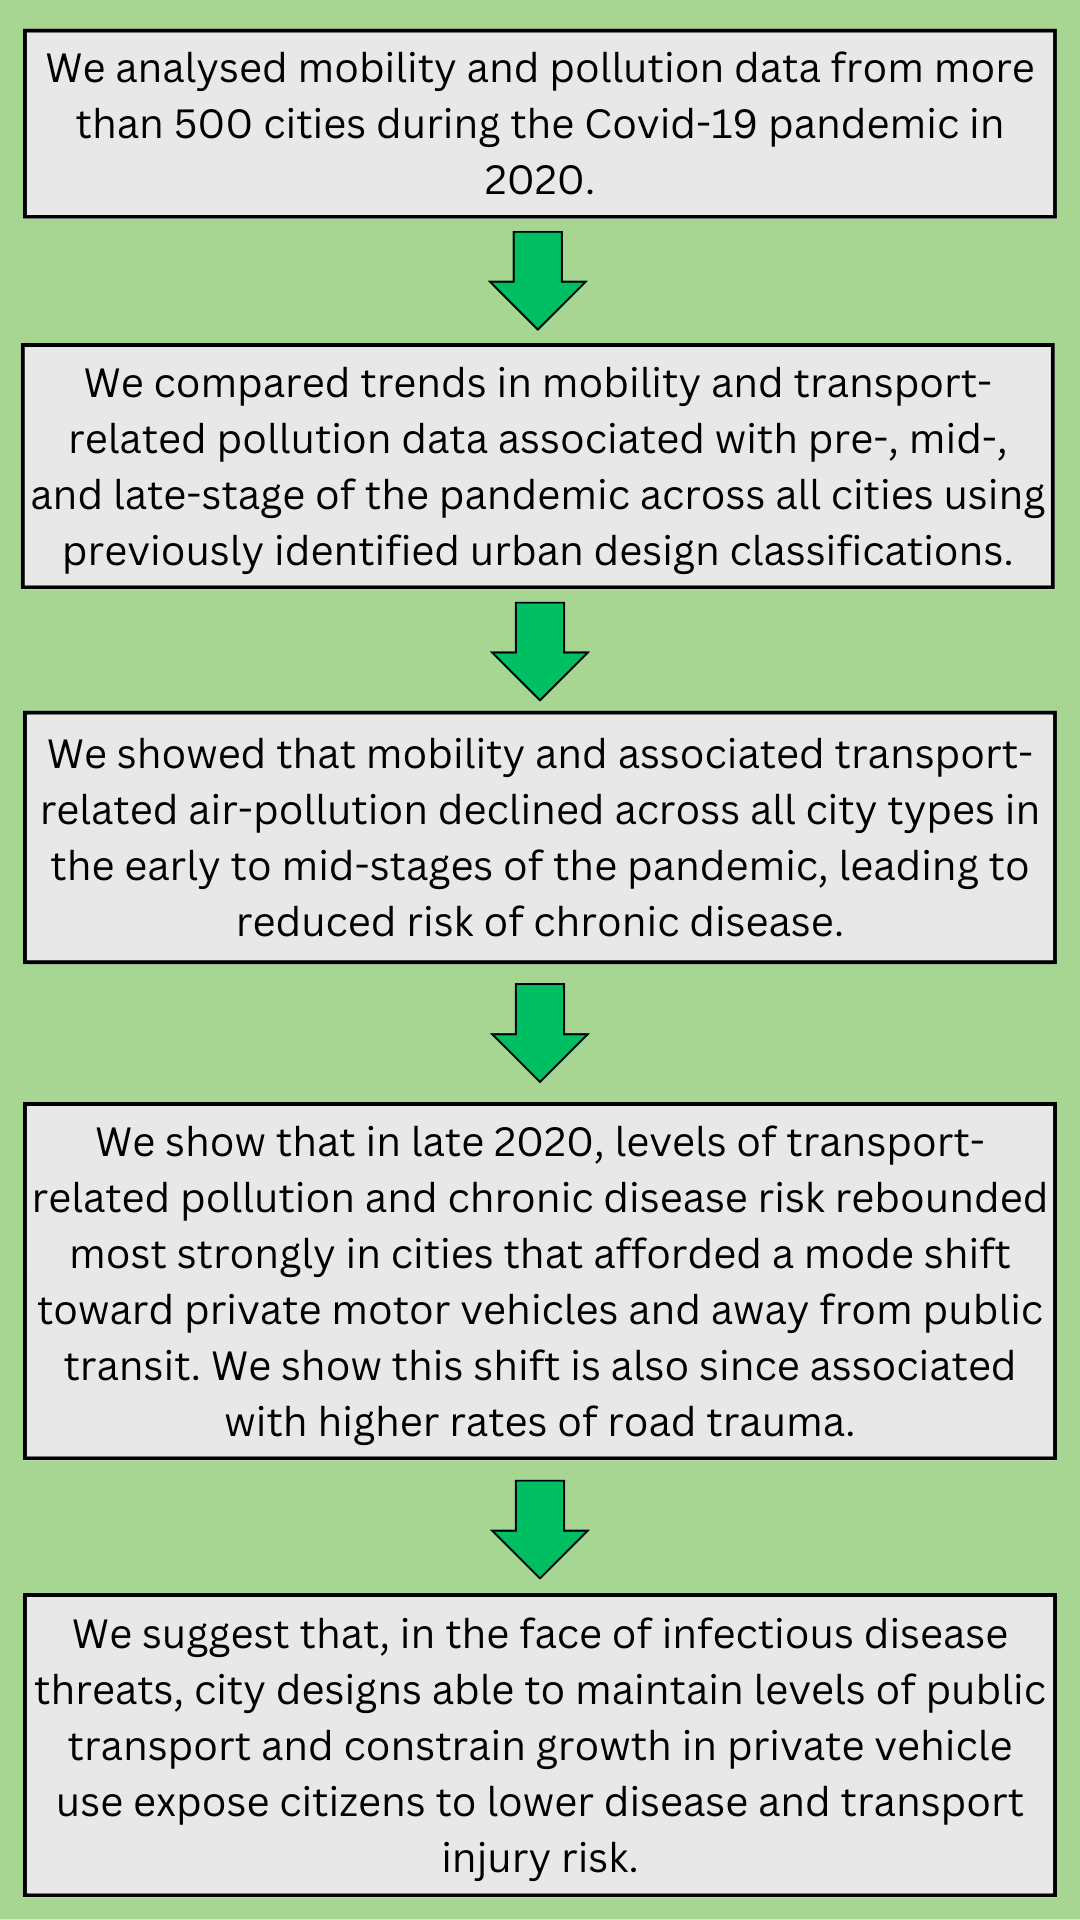
\includegraphics[trim={ 0 0 0 0 },clip,scale=0.35]{Images/Panel LPH.png}
\caption{\bf The conceptual model for the study, combining mobility and pollution data for 500 global cities during 2020 to demonstrate city design can enable or constrain public health measures leading to either better or worse disease and transportation injury risk.}
 \label{fig:concept}
\end{figure}

\section*{\textcolor{OliveGreen}{Global analysis of responses to a public health crisis}}

Starting with 1692 global cities (all cities with populations exceeding 300,000 and had available spatial data\cite{UNDESA2019}), datasets were assembled and analysed to explore city designs and pollution over time. These datasets include the network structures of urban transportation systems, historic and predicted pollution levels, mobility indicators across 2020, measures of individual disease transmission in 2020, and measures of structural dimensions of each individual city's design.

\subsection*{Characterisation of city design}
The first stage of this research was to create a representation of cities that accurately captured features of city design related to city mobility and public health. Analysing urban design centred around urban road networks has previously been undertaken in a number of ways, such as generating metrics of the `three Ds'\cite{Ewing2010}, density, diversity, and design (later updated to also include destination accessibility and distance to transit). Barthelemy (2011)\cite{Barthelemy2011} uses graph networks to derive measures of betweenness centrality, closeness, and connectedness between nodes of the network graphs. Here, we utilise a graph neural network (GNN) (see Box \ref{box:gnn}) constructed utilising OpenStreetMap (OSM) road network data\cite{Boeing2017a} from a set of 1692 global cities above 300,000 population, previously identified in Thompson et al. (2020)\cite{Thompson2020}. Due to lack of available pollution data in many cities (limitation in data was typically from low income countries in the global south), the final set of cities was reduced to 507 (Figures \ref{fig:africa}-\ref{fig:southhamerica}). The graphs generated for the GNN consist of nodes (intersections) and edges (roads) to which we have attached annotations to the edges (including road types such as residential, secondary, or arterial, speed limits, length and shape of the roads, and additional characteristics such as one way or the presence of footpaths or bike lanes) and to the nodes (node locations in reference to other nodes and the number of and angles of intersecting roads). As a result, the GNN can capture well the topography of a city's transportation networks as well as broader characteristics such as compactness vs. sprawl or symmetry vs. irregularity.  

% script is /mnt/New4tb/data/LancetPH/LPlH-Rev2/plot_Figure1.py
\begin{figure}
\centering
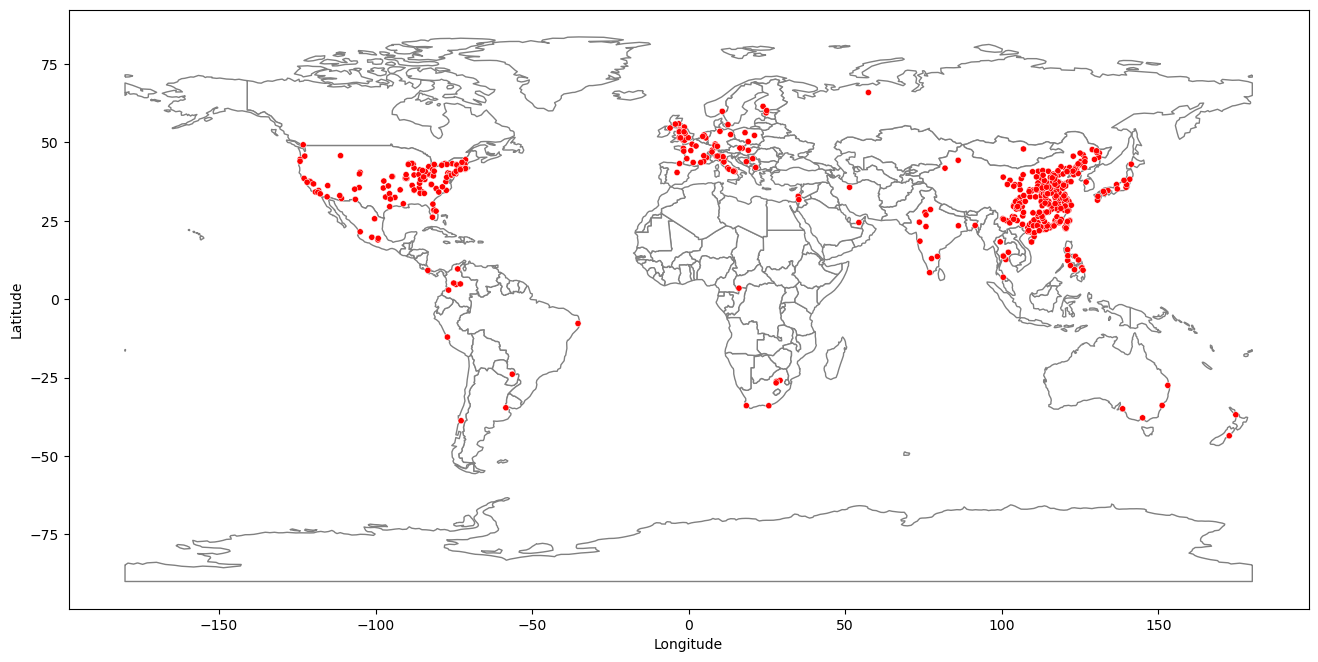
\includegraphics[trim={0 0 0 0},clip,scale=0.4]{Images/ByCountry_map_Black.png}
\caption{\bf Location of the 507 cities used in this study.}
 \label{fig:clusters}
\end{figure}

City-level air pollution data (see Box \ref{box:pollution}) was used to validate the representation learned by the neural network. For each city, the neural network could predict whether air pollution levels rose or fell compared to the previous year with an accuracy of 97\%. This result underscores the neural network's ability to not only capture the road network of the modelled cities, but also to approximate the relationship between the transport network and the behaviour of air pollutants within the city. Additional validation of the neural network comes from Figure \ref{fig:Dimensions}, which plots the t-SNE representation (see Box \ref{box:gnn}) against understood dimensions of urban design measured against city block size and block regularity (i.e., the extent to which city blocks form parallelograms), as well as percentage of road and transit networks observed in each city from prior studies\cite{Thompson2020,Nice2019b}. Combined with Figure \ref{fig:clusters} and Figure \ref{fig:tSNE}, Figure \ref{fig:Dimensions} demonstrates that the urban morphology for analysed cities follows gradual changes across dimensions. High-density, small-block size and cities with relatively regular (e.g., quadrilateral) blocks are depicted on the mid- to upper-left of Figure \ref{fig:tSNE} (e.g., in grid areas A2/A3 and B1/B2), whereas sparse, large-block cities with little public transit infrastructure as a proportion of the transport network cluster together in the bottom right through areas G7 to H6. 

Figure \ref{fig:tSNE} also shows that cities from within countries and continents tend to cluster together. For example, Japanese cities tend to cluster tightly together across grid areas A3 and A4, while European cities cluster together in and around grid areas A2 to C4. Asian cities across China, India and Vietnam extend in a regular pattern from grid areas B5 through to H6 as their designs differed along dimensions of block size and road network density. Of note are also clusters of Australasian, South American and North American cities found in grid areas C1 to C3 and B1 to B3. Urban designs in these areas tended to demonstrate regular, medium-sized blocks with medium to low levels of public transit. Cities in these locations were typically of a `Chequerboard' (square blocks) or `Motor City' (large, oblong blocks) types, designed to facilitate the egress of motor vehicles.

\subsection*{Reductions in air pollution and associated health outcomes during the COVID-19 pandemic}
Much research has explored the association between air pollution (e.g., NO$_{2}$, PM$_{2.5}$, O$_{3}$, and PM$_{10}$) and health outcomes. In general, this work has indicated that the dose-response relationship between pollutants and health outcomes (e.g., disease incidence, hospital presentations, etc.) is generally linear, with no evidence of a threshold~\cite{schwartz2002concentration}. We estimated risk reductions within each of the pandemic's `Entry' (12.1\%), `Mid-Crisis' (45.8\%), and `Recovery' (31.2\%) phases of the crisis across each of 5 regions and globally,  defined as between days 1 and 46, 47 to 83, 84 to 250, and day 251+, respectively (phases begin Jan. 1, Feb. 16, Mar. 24, and Sep. 7) . 

Associations between air pollution at the city level and estimated health risk effects were made for NO$_{2}$ across all-cause mortality, cardiovascular disease, and respiratory disease \cite{Huang19Pollution}. Similarly, changes in PM$_{2.5}$ pollution levels were associated with estimated changes in relative health risk for all-cause mortality, ischaemic heart disease mortality, and asthma consistent with contemporary estimates \cite{Xie257, Yu2020PM2.5, BALTI2014161} (i.e., \( \mathrm{RR} = 1 + \frac{\text{risk coefficient} \cdot \text{anomaly}}{units of pollution variable (e.g., 10)} \)). 

% script is /mnt/New4tb/data/LancetPH/LPlH-Rev2/plot_Figure1.py
% now is plot_Figure2Revised_flags.R
\begin{figure}
\centering
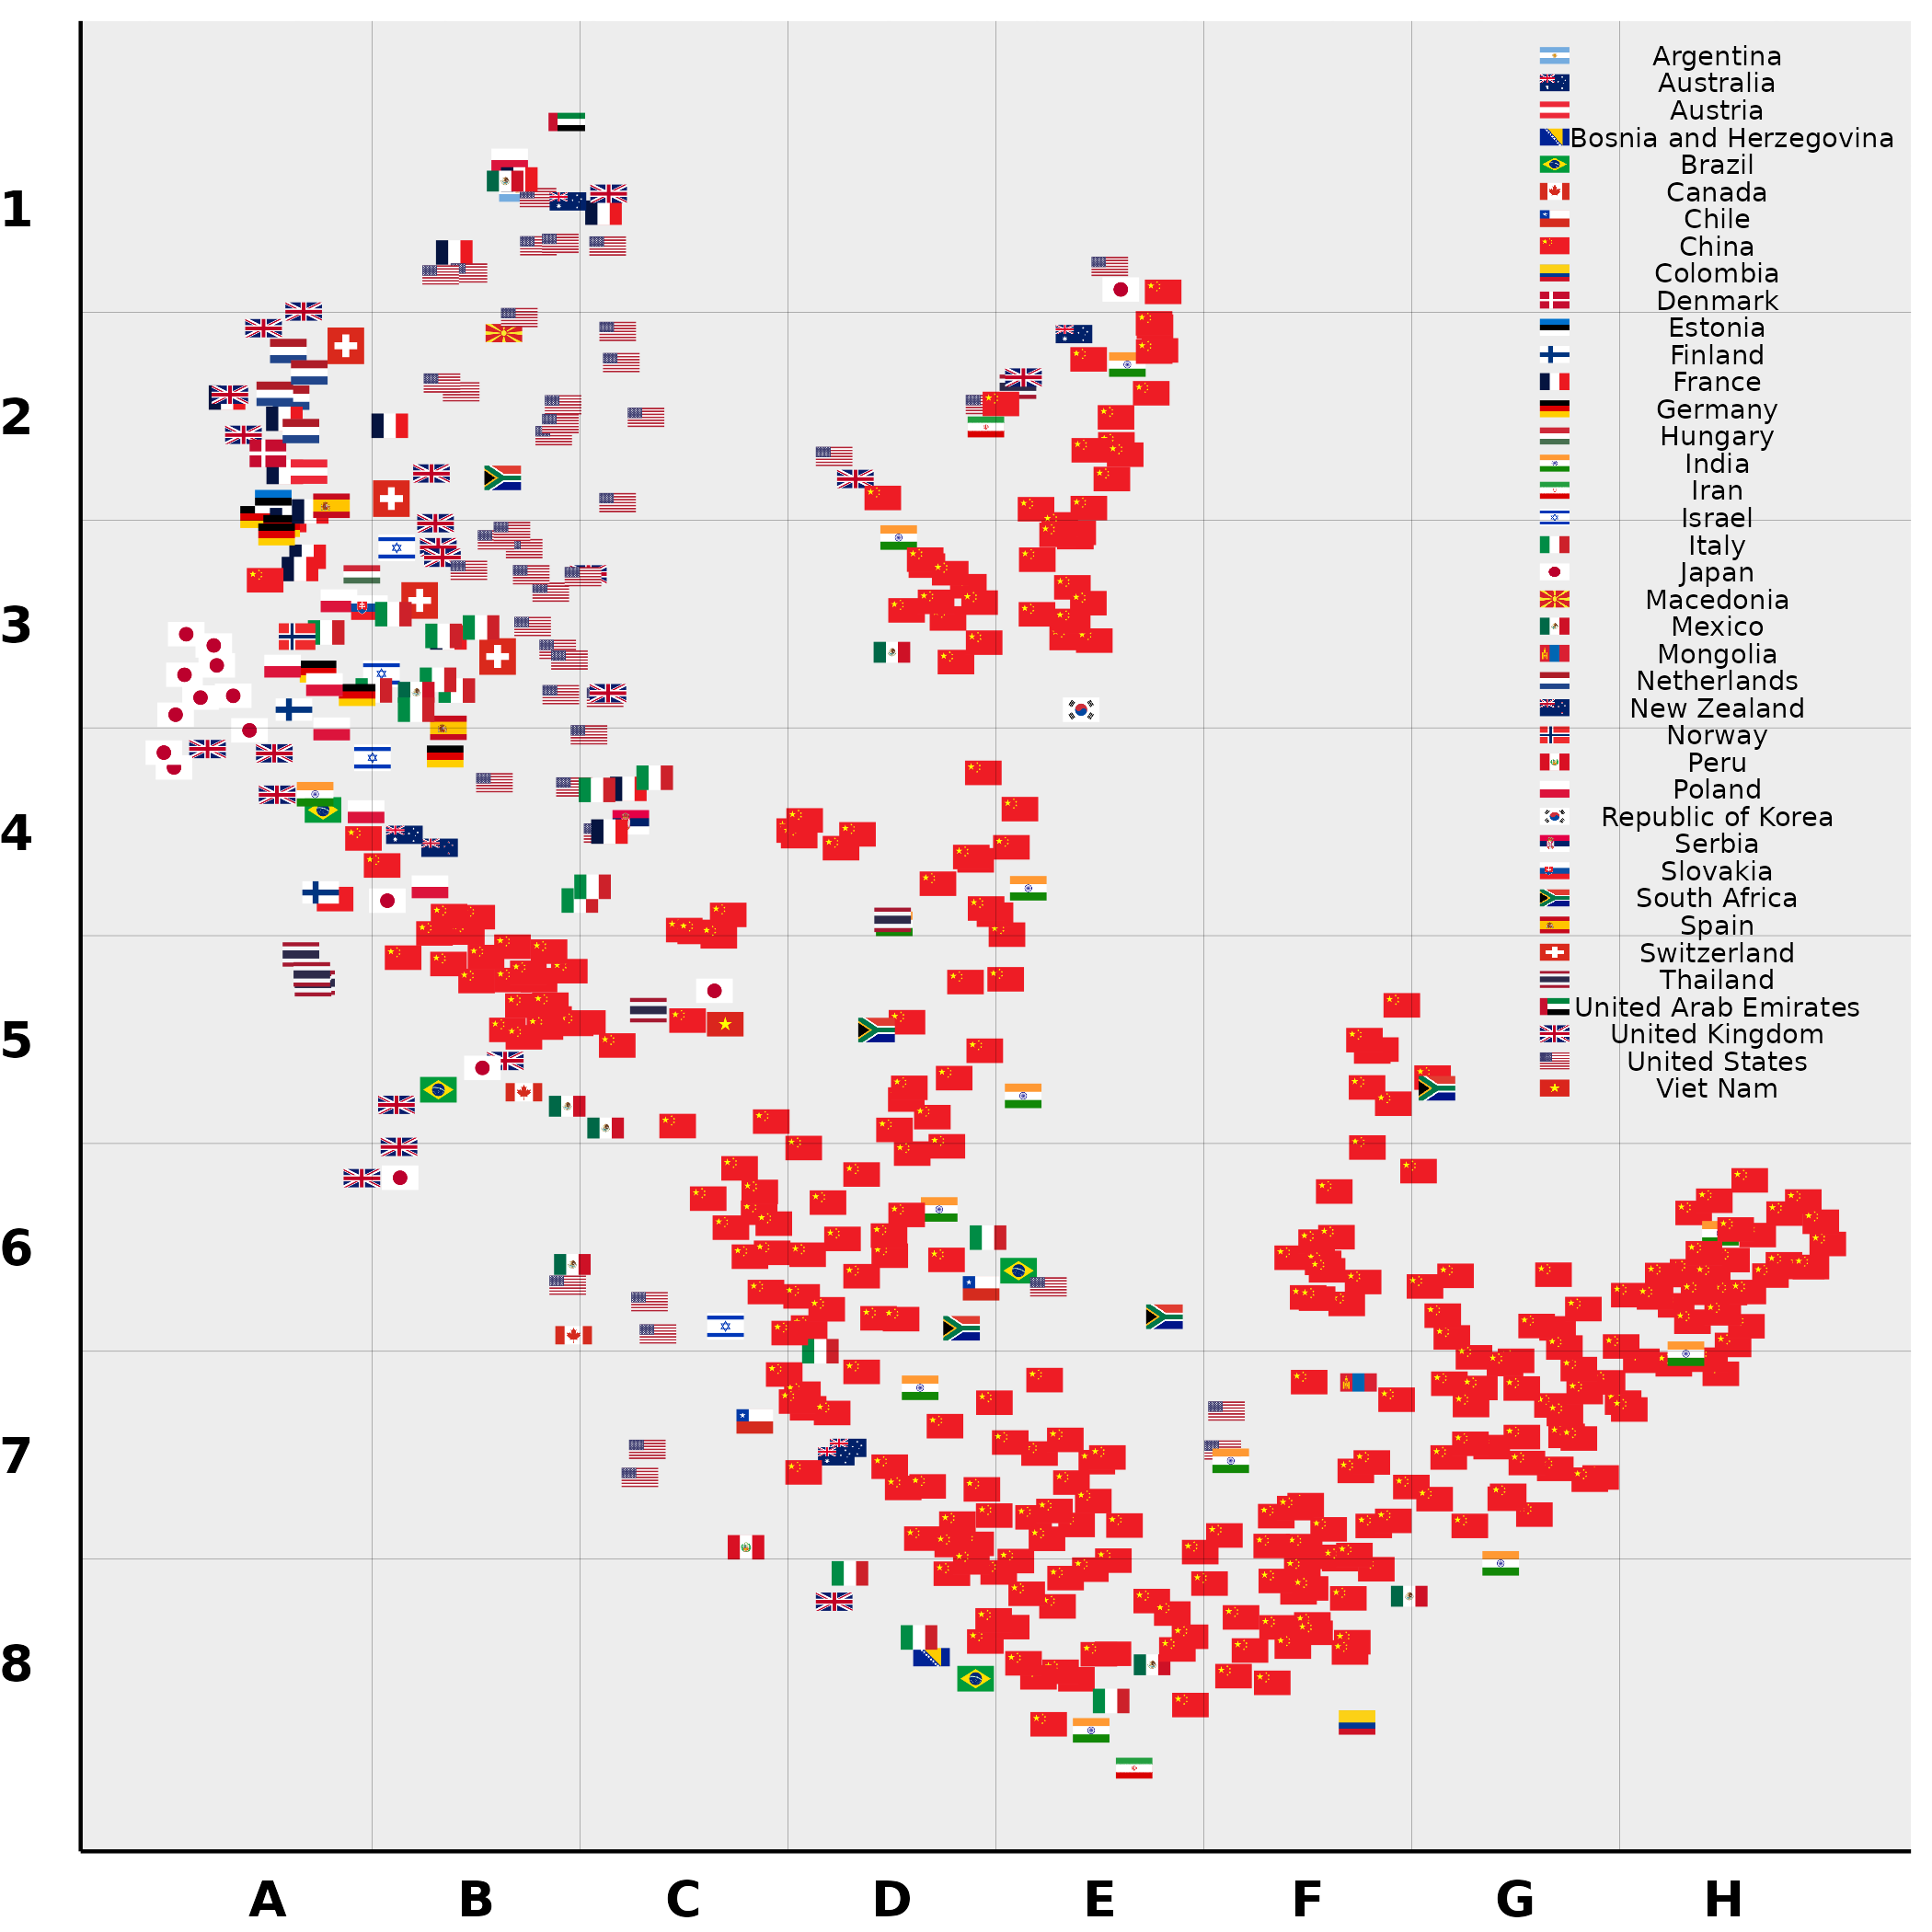
\includegraphics[trim={ 0 0 0 0 },clip,scale=1.0]{Images/ByCountry_latlong_flags_all.png}%tSNE Country.png}
\caption{\bf t-SNE 2-dimensional representation of 507 global cities, organised by similarities across urban characteristics from OpenStreetMap network graphs. Grid references (i.e. A1) are used in the text to describe regions in the graph.}
 \label{fig:tSNE}
\end{figure}



%script is now plot_Figure3Revised.R
\begin{figure}
\centering
\scriptsize{a)} 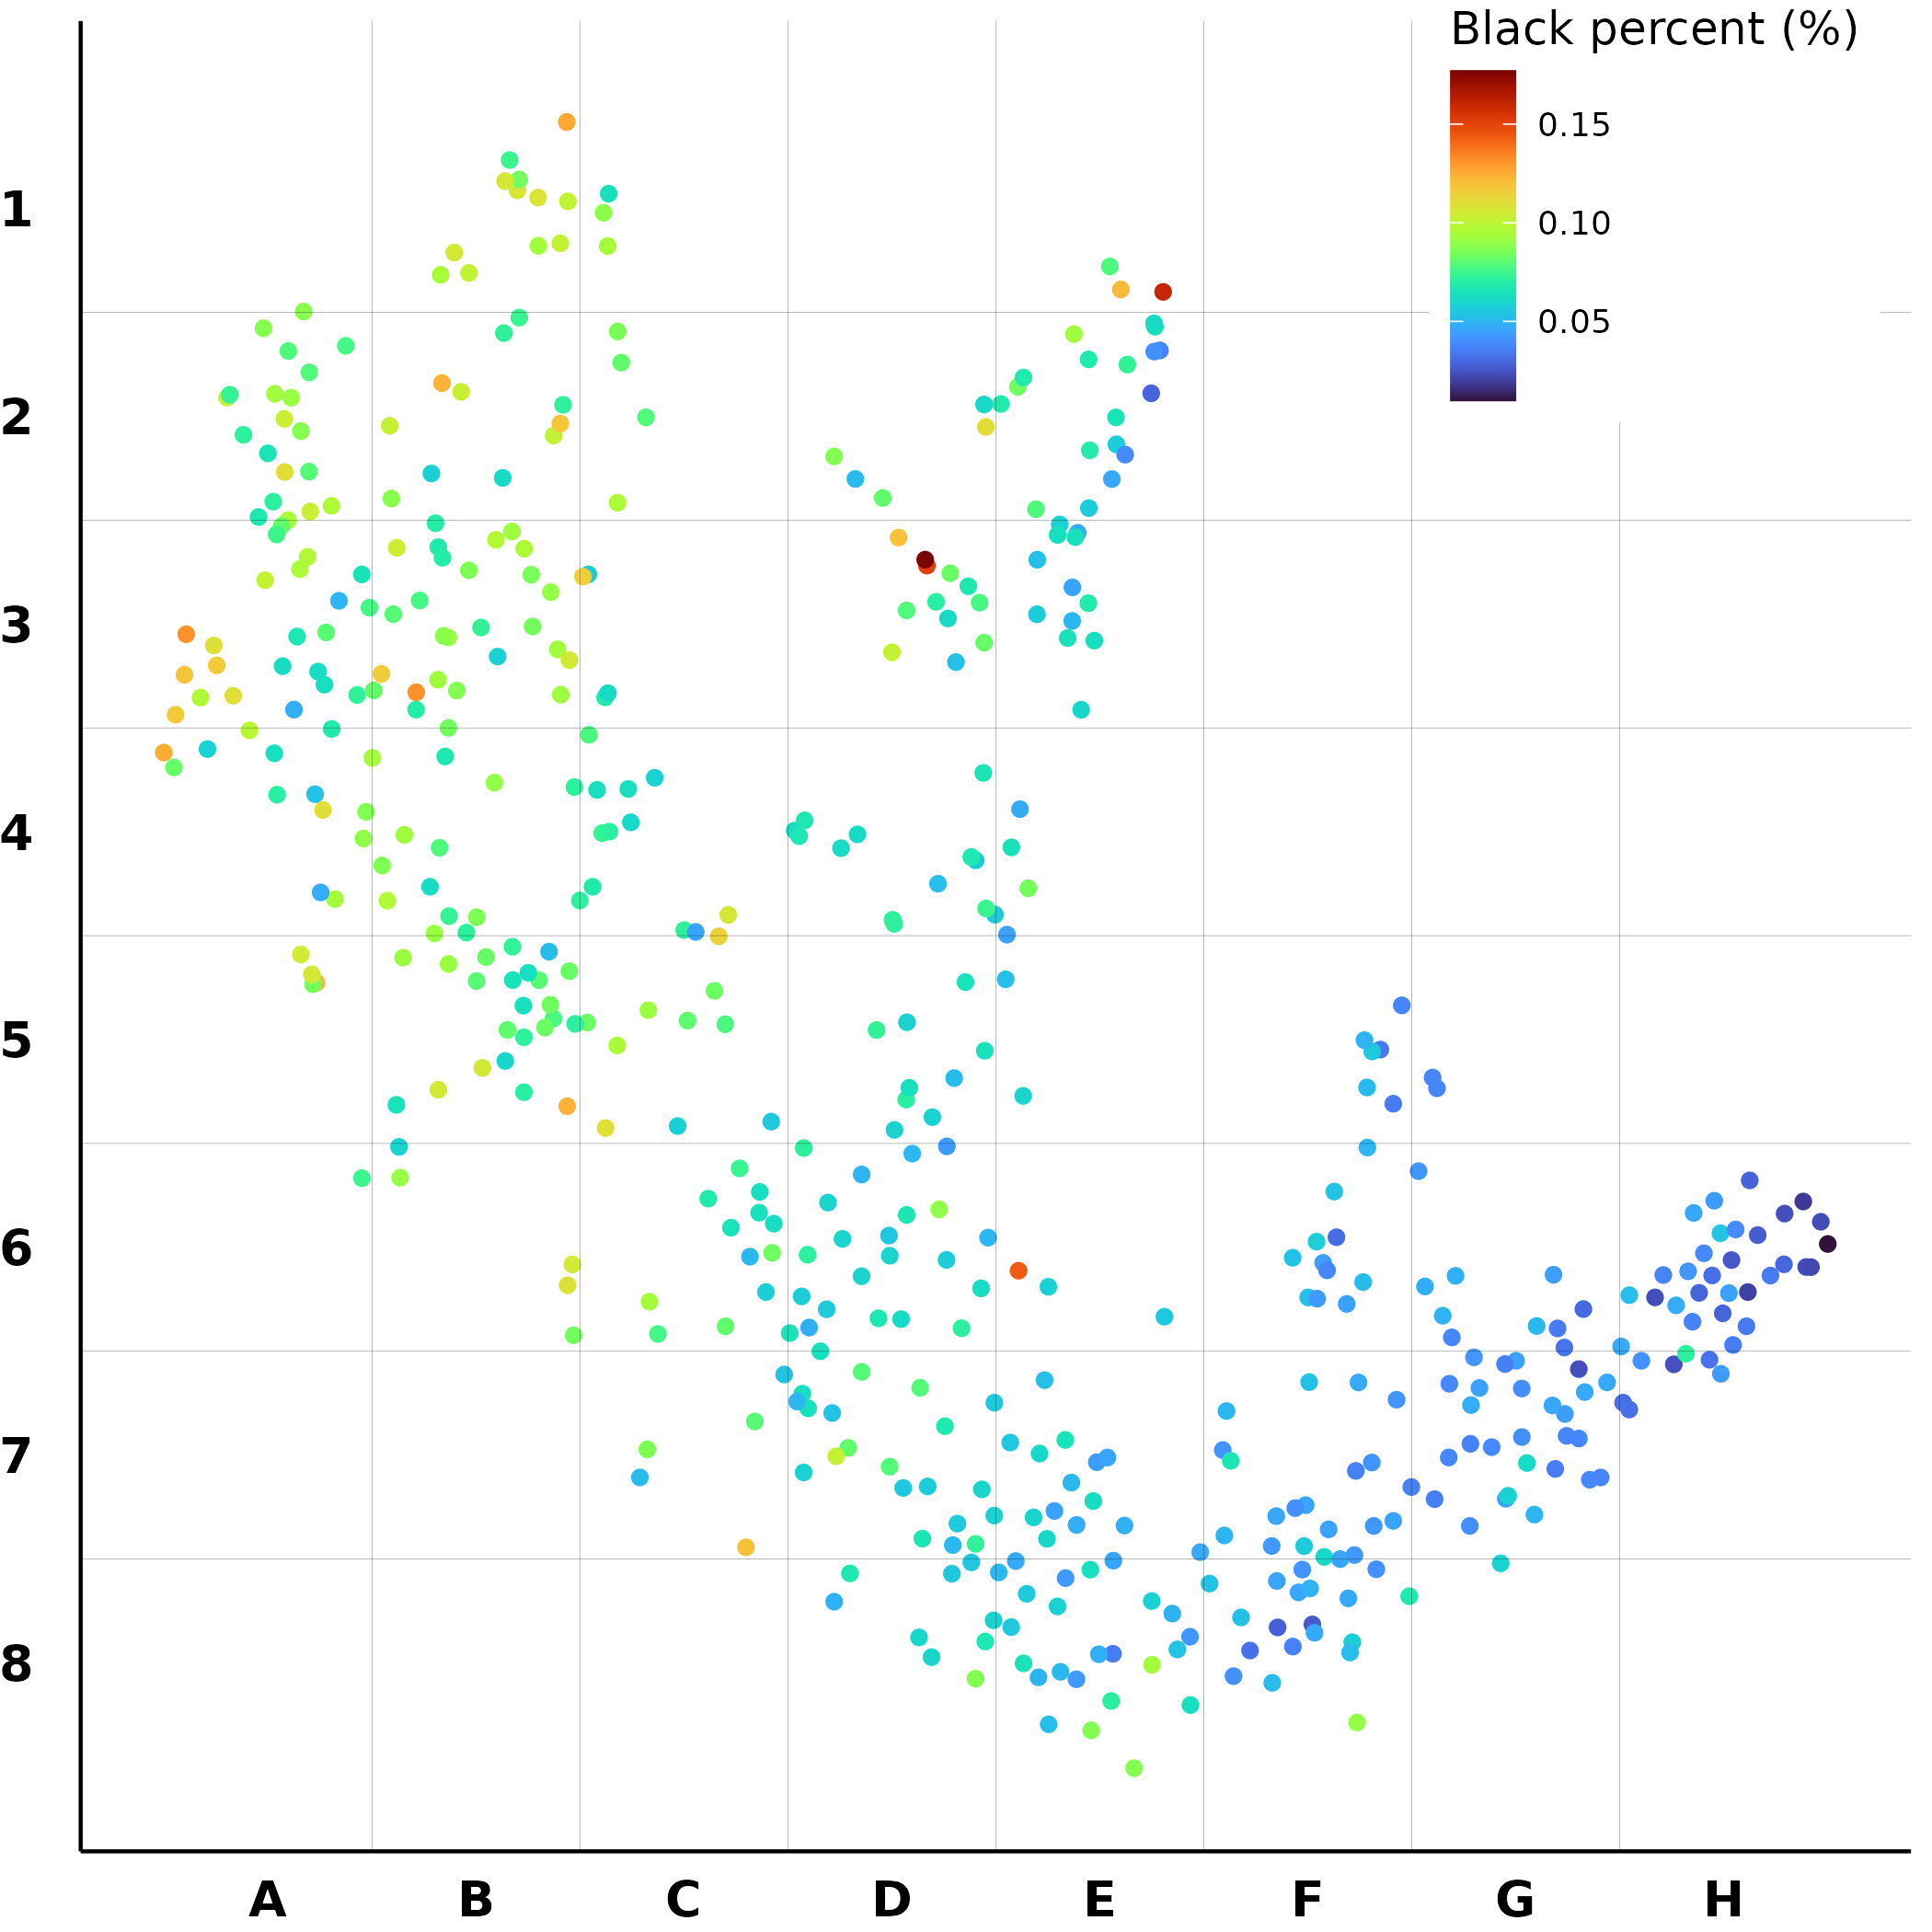
\includegraphics[trim={ 0 0 0 0 },clip,scale=0.35]{Images/City_Types_Dimension_chessboard_blkPct.png}
\scriptsize{b)} 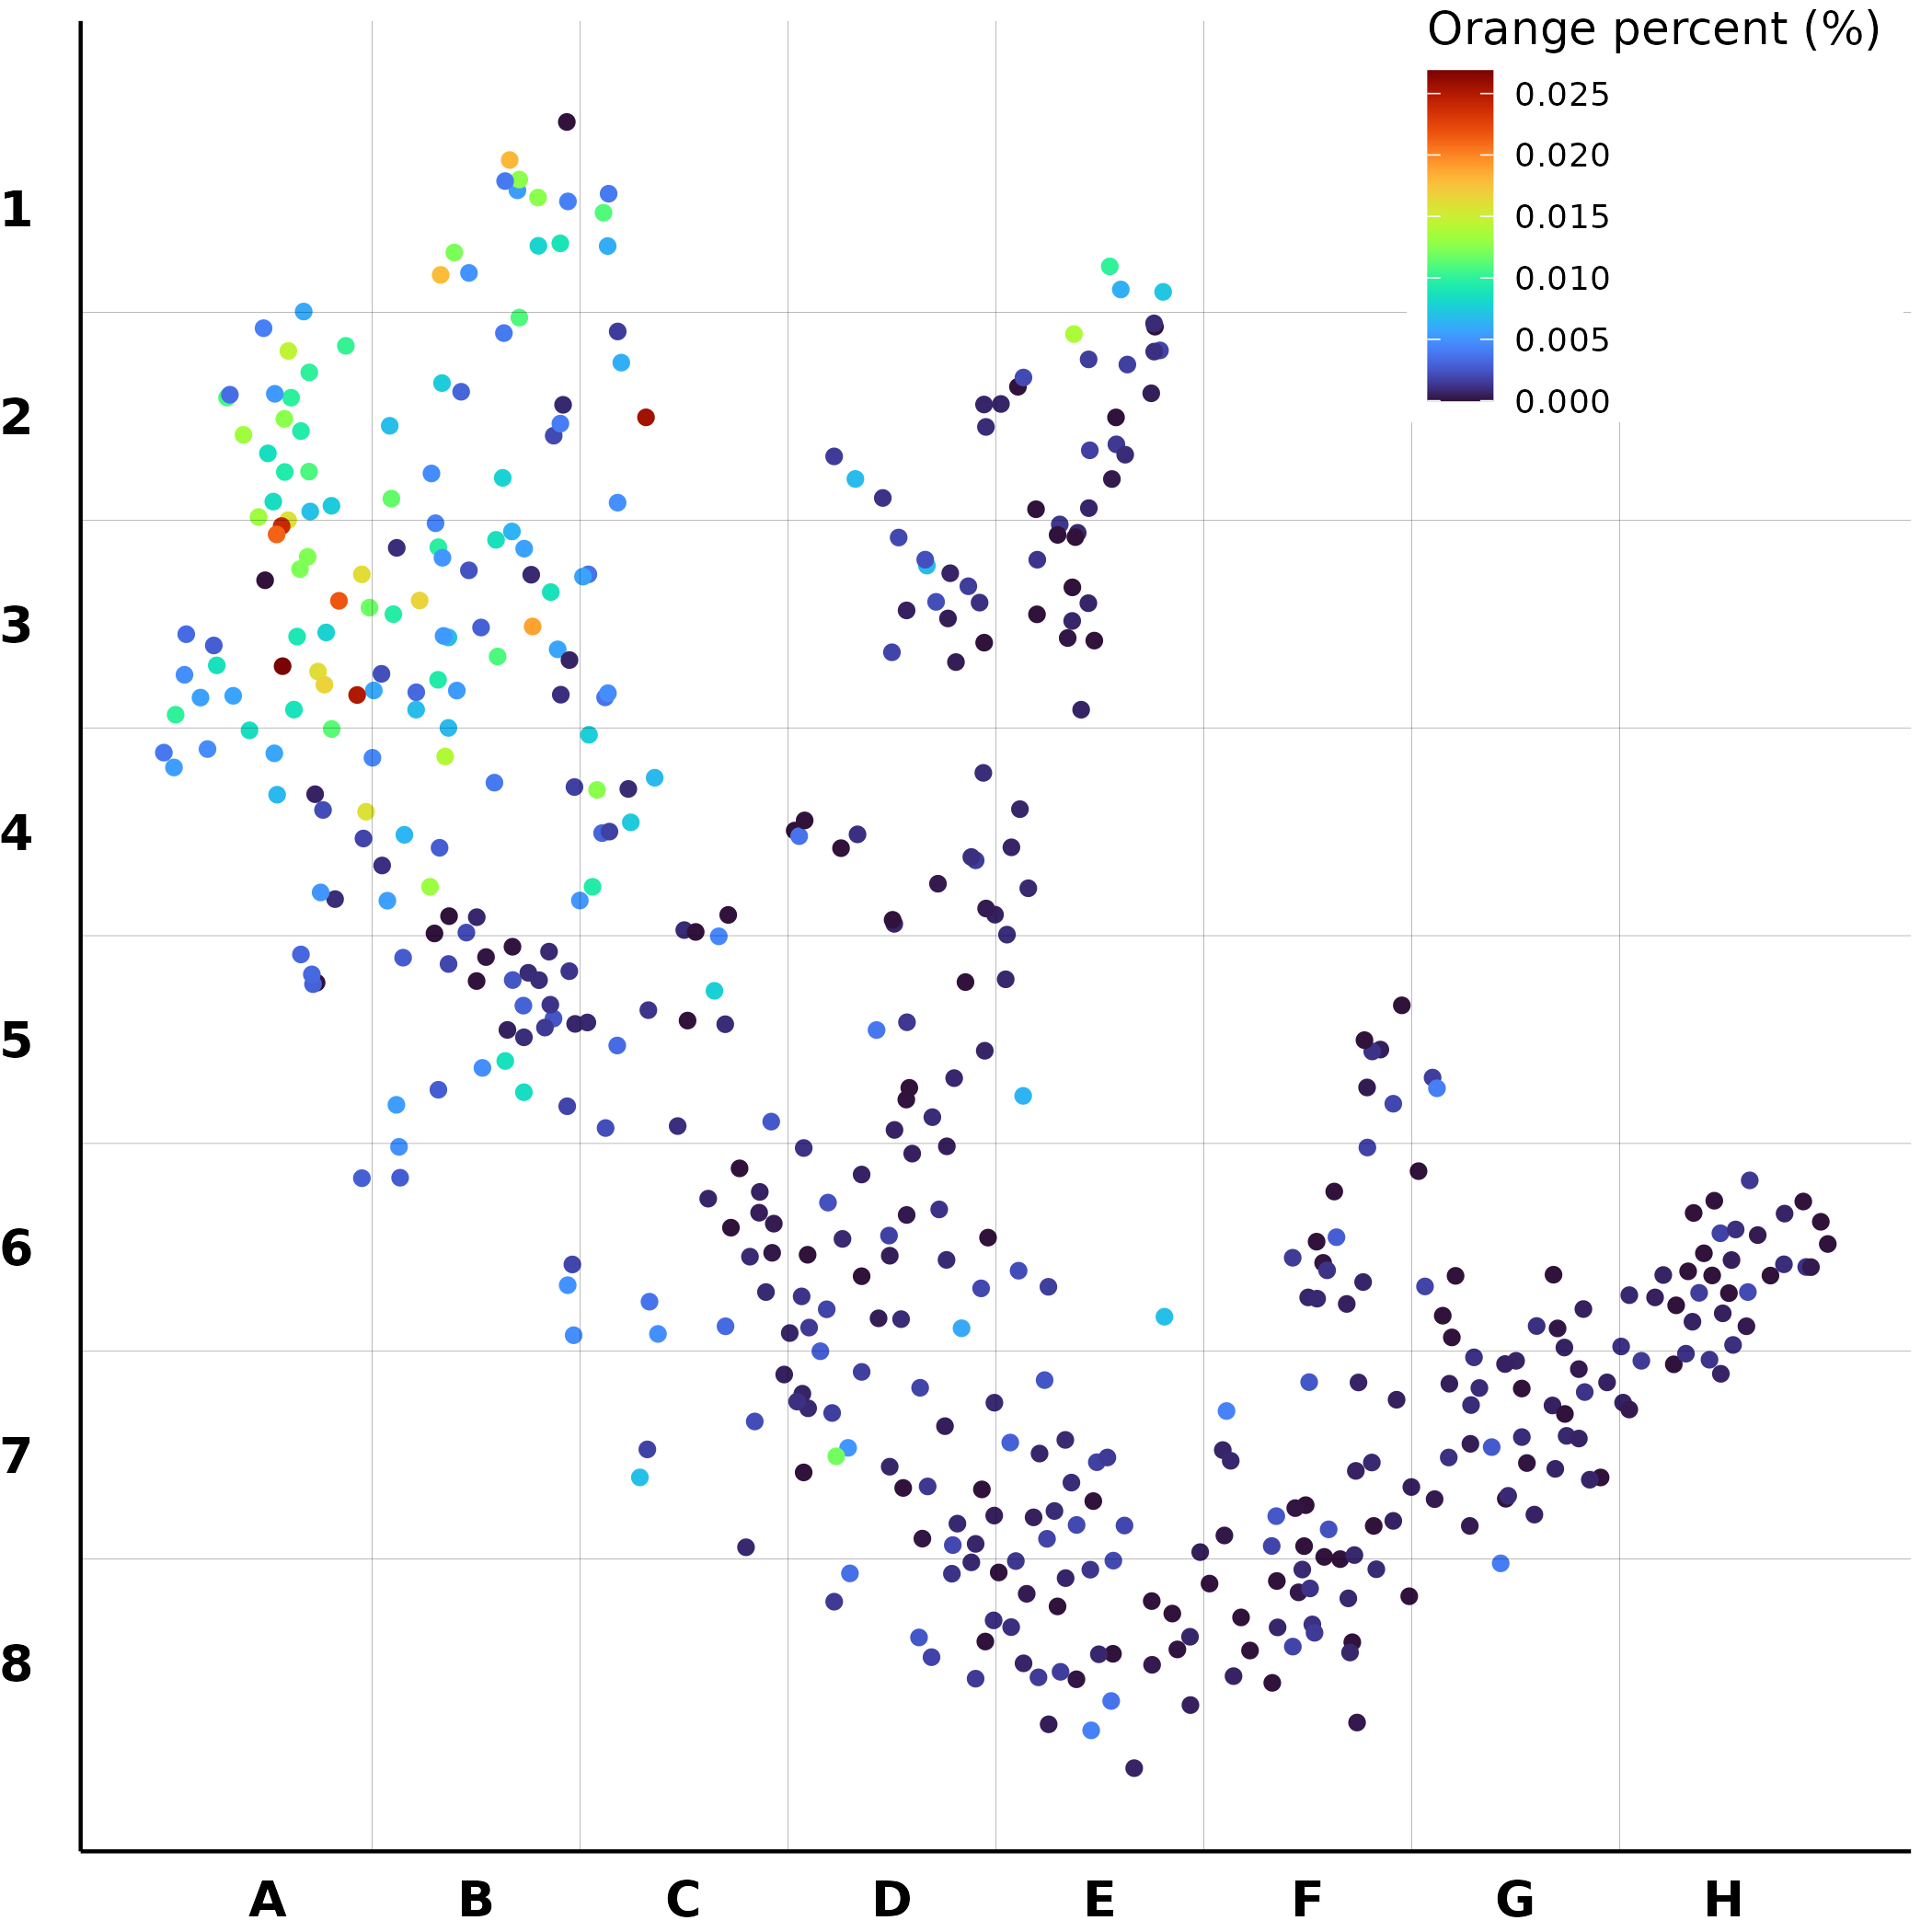
\includegraphics[trim={ 0 0 0 0 },clip,scale=0.35]{Images/City_Types_Dimension_chessboard_orangepct.png}
\\ \scriptsize{c)} 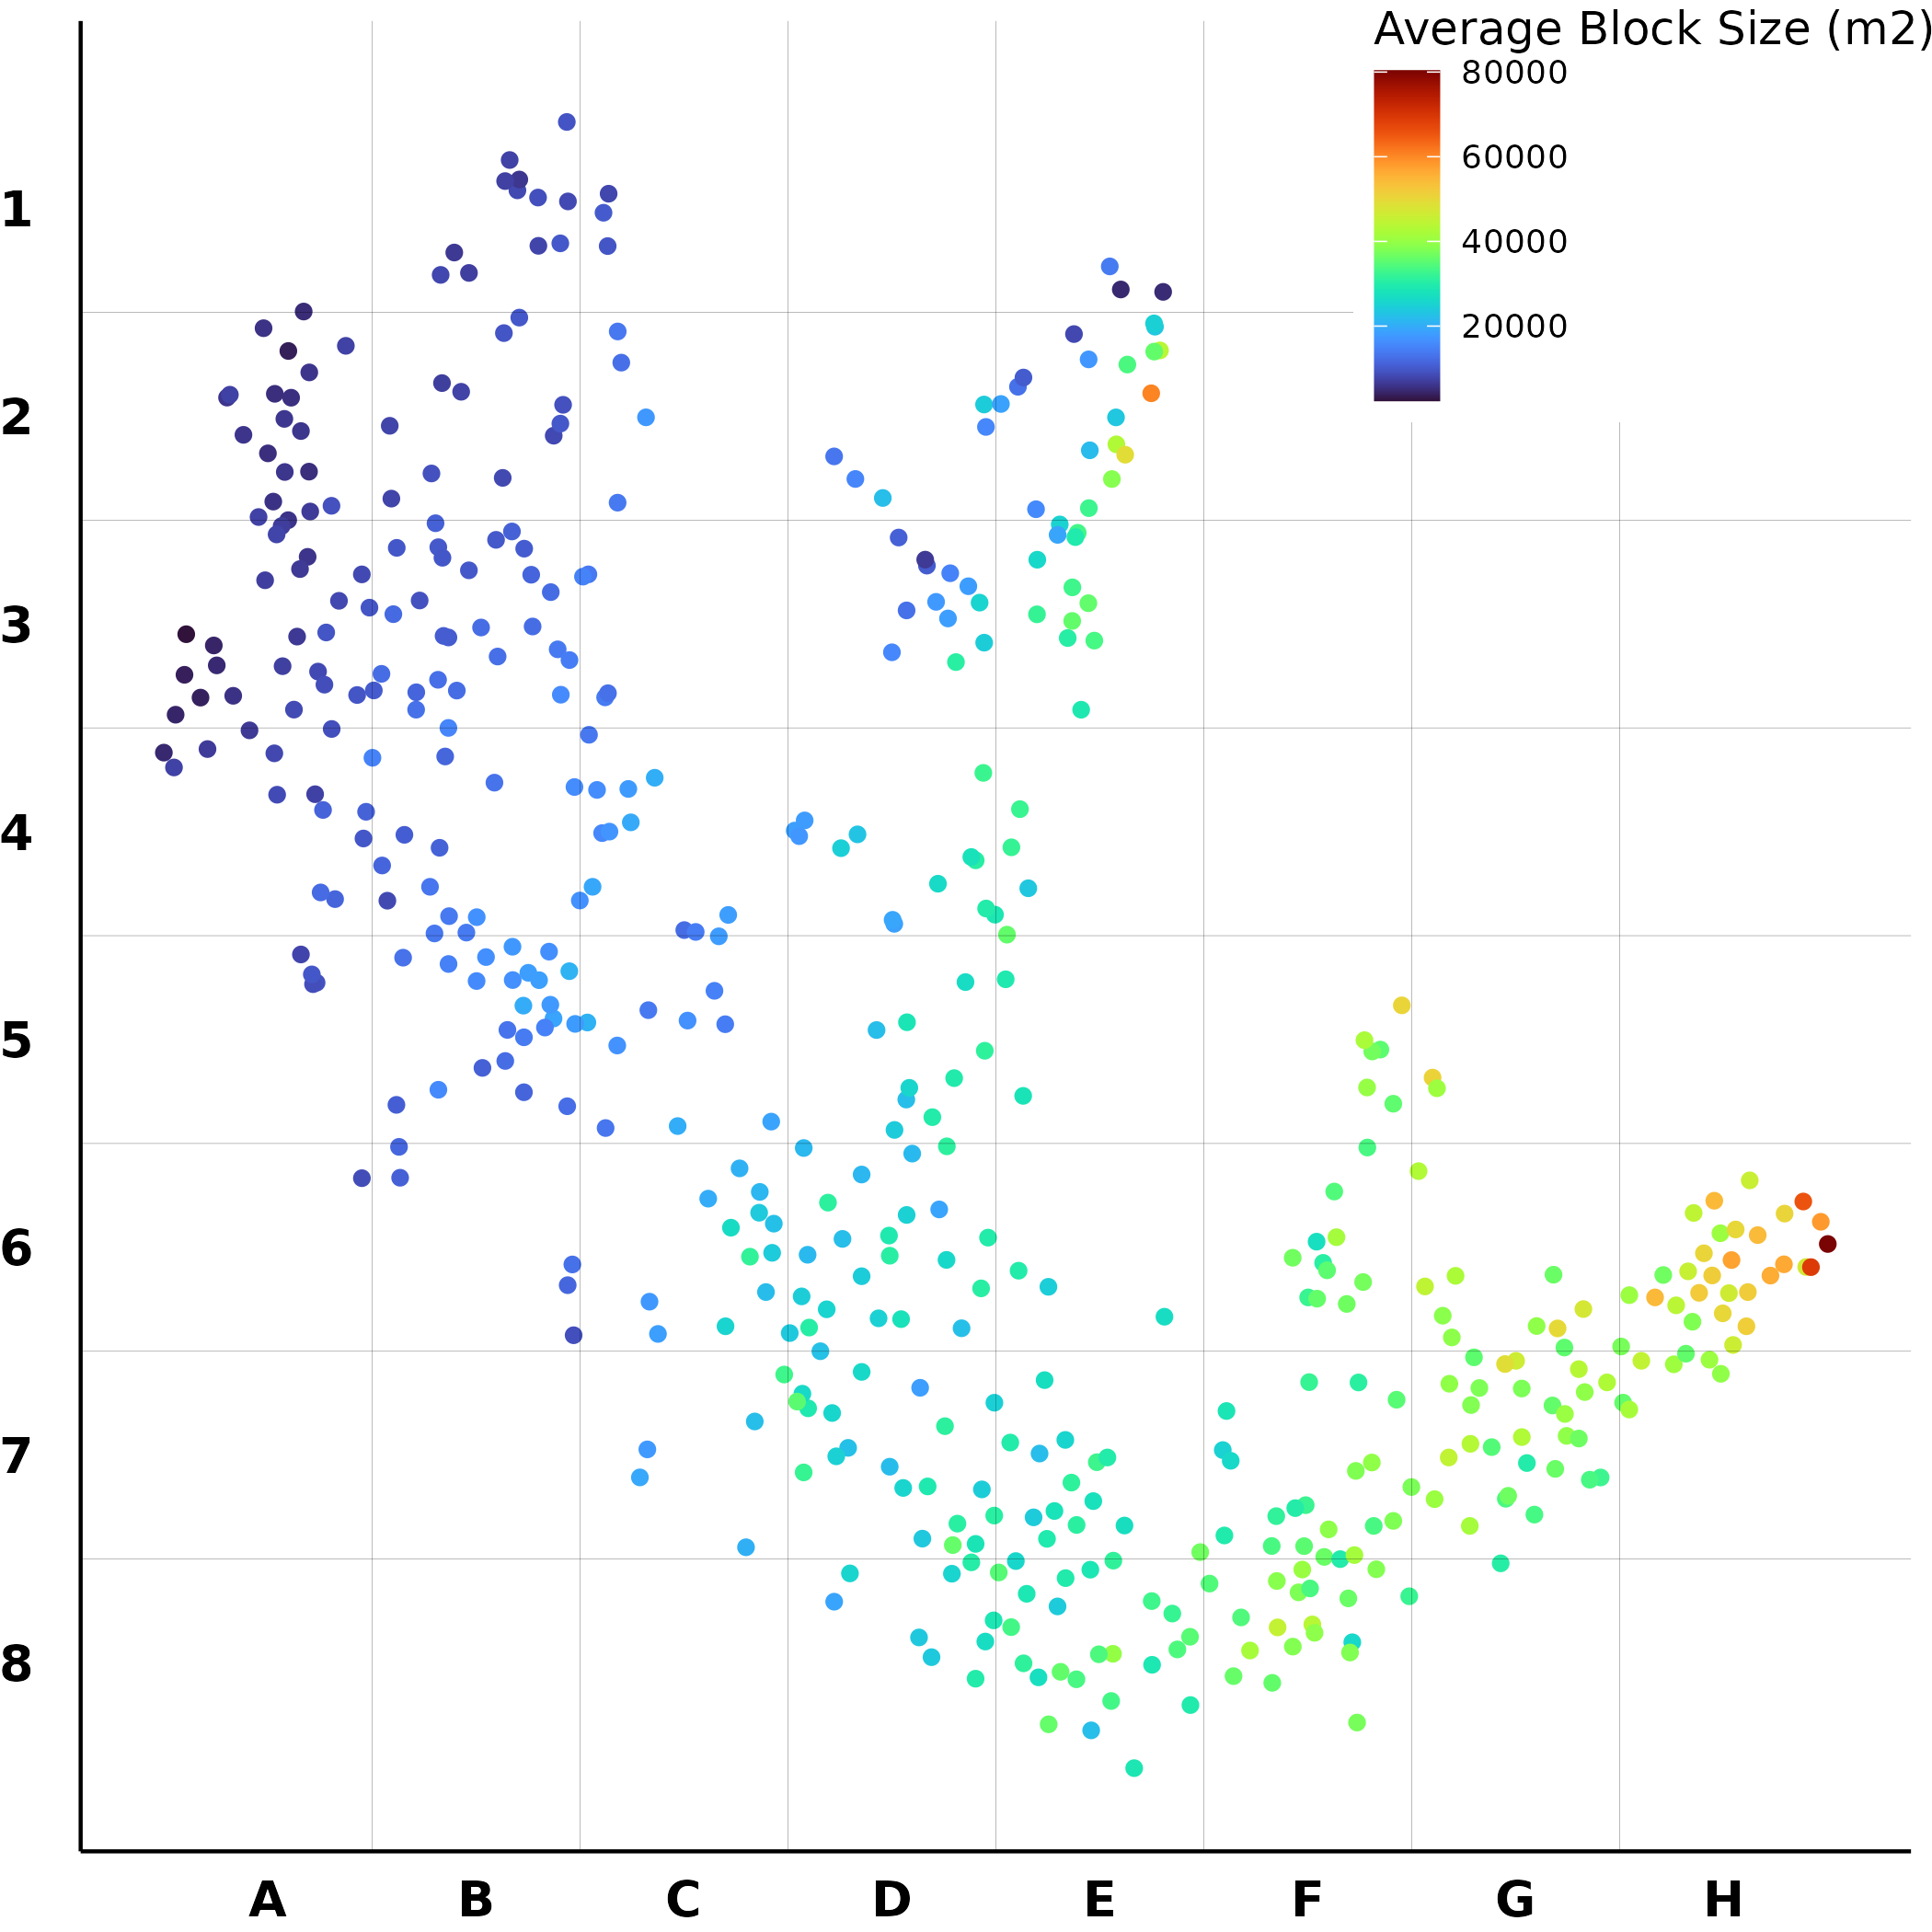
\includegraphics[trim={ 0 0 0 0 },clip,scale=0.35]{Images/City_Types_Dimension_chessboard_AverageBlockSize.png}
\scriptsize{d)} 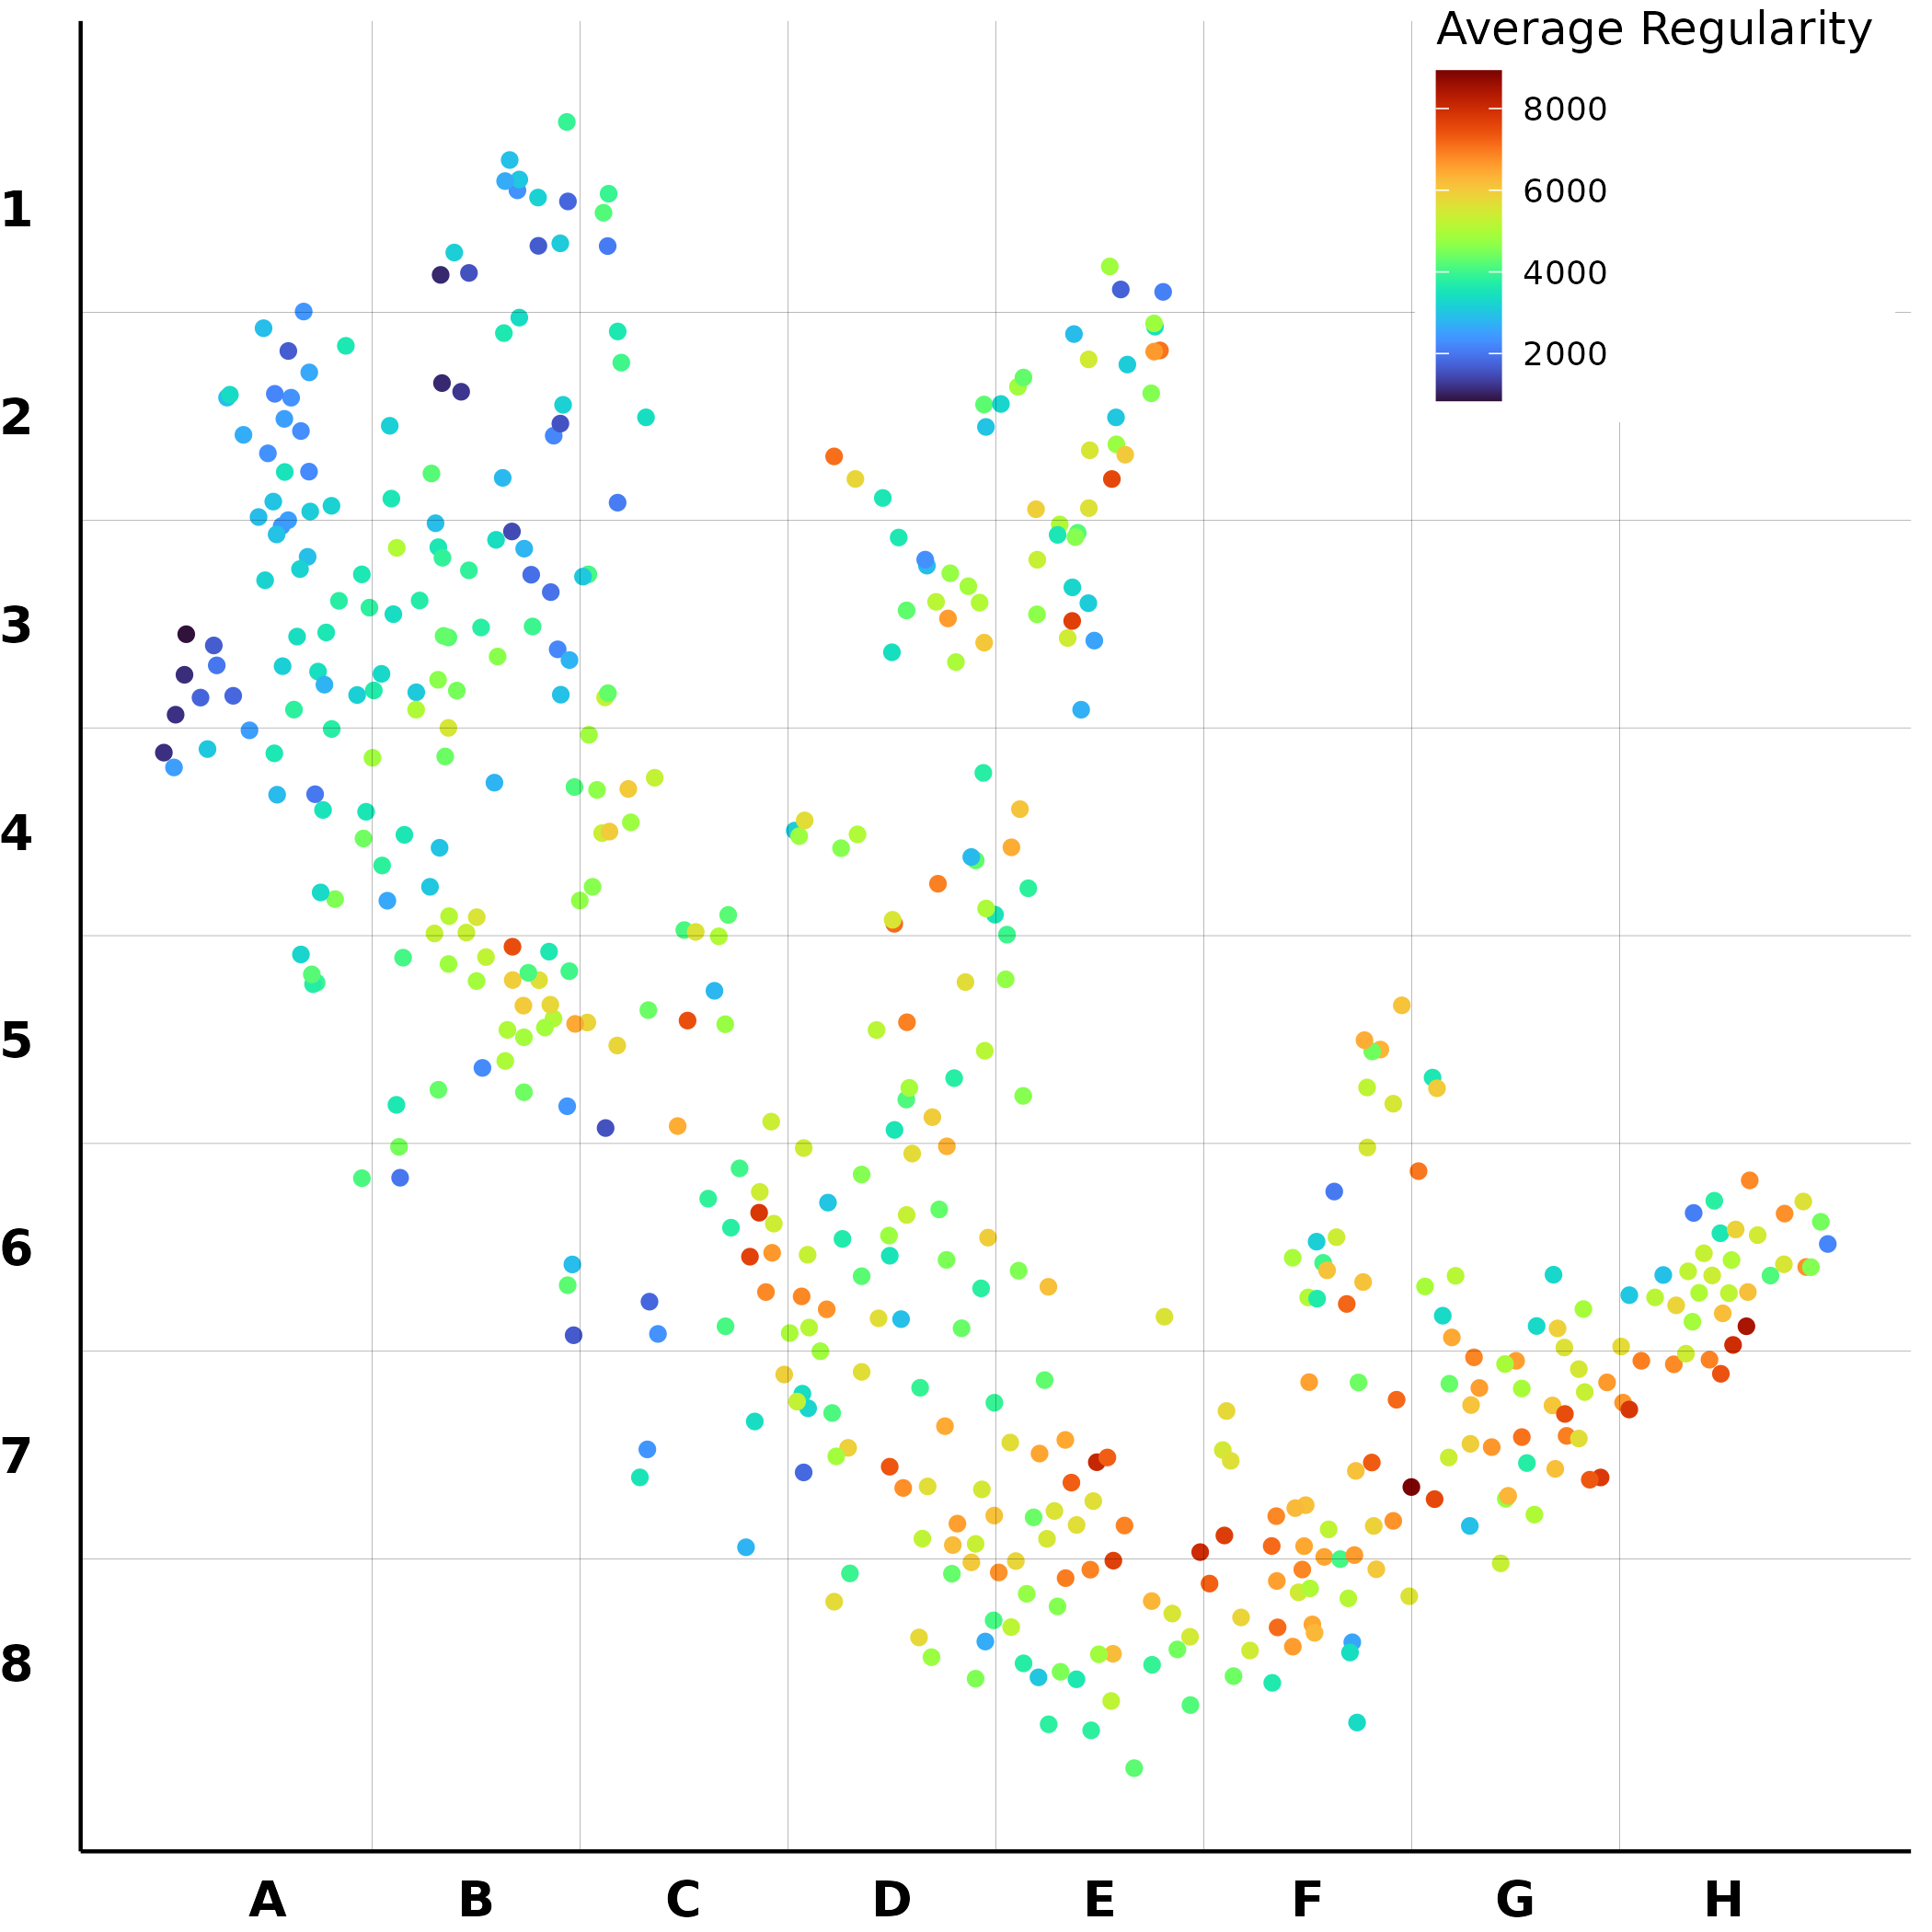
\includegraphics[trim={ 0 0 0 0 },clip,scale=0.35]{Images/City_Types_Dimension_chessboard_AverageRegularity.png}
\caption{\bf Characteristics of 507 global cities (from Figure \ref{fig:tSNE}) showing percentages\cite{Thompson2020} of a) black and b) orange pixels from sampled maps, reflecting amounts of road space and public transport rail lines in each city. Panels c) and d) show\cite{Nice2019b} average block sizes (m$^{2}$) and a measure of city block regularity (lower values reflect increasing squareness). City locations and grid references correspond to those in Figure \ref{fig:tSNE}}
 \label{fig:Dimensions}
\end{figure}


\begin{figure}
\fbox{\parbox{\textwidth}{
Growing availability of spatial big data have led to increasing usage of graph neural networks (GNN) in urban studies, using urban street networks to explore the urban form, discover urban growth patterns and socioeconomic statuses, derive the functions of urban features in street view imagery, or to enable the fusion of multiple sources of information to uncover the cultural characteristics of neighbourhoods from street view imagery \citep{liureview2022,desabbatalearning2023,xuequantifying2022,zhangknowledge2023,silvausing2024}. GNNs work by forming high-dimensional hypotheses that can represent input data; in this case, road networks, public transit networks, and active transport networks (e.g., walking and cycling paths) derived from OSM data. In the context of understanding mobility patterns, the utilisation of OSM data offers significant advantages over sampled imagery data used in previous studies (e.g.\cite{Thompson2020,seneviratne2021self}) due to OSM data's high density and its capacity to represent features of an entire city, rather than relying upon sampled data from locations across cities. To conduct global studies, OSM has proven to be an essential source of data, especially in data poor regions of the world where it might be the only source of that information. Assessments have found that while OSM data might have lower levels of completeness, the accuracy is generally high \cite{Zhou2022c,Zhou2022d}. OSM data was gathered in March 2023, so might have some differences between the study period (2020). However, as road and transport networks do not change dramatically over short periods \cite{Taillanter2023} makes it less likely that major infrastructure changes took place during that period and the lag time ensures that volunteer-run updates of OSM would likely have caught up with recent infrastructure changes. Furthermore, in comparison to the use of imagery data, the analysed road networks of each city present a direct, rather than inferred, data source. The coverage of cities analysed are shown in Figure \ref{fig:clusters} and Figures \ref{fig:africa}-\ref{fig:southhamerica}.

We trained a graph neural network using self-supervised learning; a method demonstrated to capture urban form comparably to supervised learning\cite{seneviratne2021self}. Importantly, this allows the graph neural network used here to represent the data without requiring a labelled output to the neural network, as used in a recent study\cite{Thompson2020}. Masked Auto-encoding (MAE) was used as the training objective of the graph neural network. This objective has demonstrated effective performance in neural networks across various data modalities such as graphs\cite{hou2022graphmae}, images\cite{he2022masked}, graphs represented as images\cite{seneviratne2022self} and text\cite{devlin2018bert}. MAE trains the neural network by `masking' part of the input data, then tasking the model with predicting the masked (unknown) portion. Here, we masked both road (edge) features--such as length, start and end locations of roads--as well as node features such as latitude and longitude. The model then attempted to predict surrounding OSM sections from the remainder of the available sample. 

The results of this analysis were then converted to a t-SNE\cite{scikit-learn} graph which organised the average value of each city's OSM sample in a 2-dimensional plane where the distance between cities on the graph represented their similarities across urban characteristics (see Figure \ref{fig:tSNE}). t-distributed stochastic neighbour embedding (t-SNE) is a method to visualise higher-dimension data by reducing it to two or three dimensions.
}}
\captionsetup{labelformat=empty}
\caption{Box \ref{box:gnn}: Graph neural network}\label{box:gnn}
\end{figure}



\begin{figure}
\fbox{\parbox{\textwidth}{
Starting with the list of the largest cities in the world\cite{UN2014}, Thompson et al. (2020)\cite{Thompson2020} classified 1692 cities into types based on urban design characteristics and the associations of these types to road transport injury. This study and Wijnands et al. (2022)\cite{Wijnands2022} also used this list as a starting point and collected data (OSM data (Box \ref{box:gnn}) and pollution data (below)), to maximise the coverage of as many of these cities as possible. 

The pollution data used in this study was derived from data generated by Wijnands et al. (2022)\cite{Wijnands2022}. That study found remote-sensing data to be of insufficient resolution (often 10km) to detect pollution anomalies of NO$_{2}$, PM$_{2.5}$, PM$_{10}$, and O$_{3}$ during 2020. Instead, ground-based observations were collected from as many locations across approximately 900 cities, supplied by the environmental protection agencies for 132 countries.  Using city-level daily averages of hourly pollution observations from 2015-2019, combined with ERA5\cite{Hersbach2020} weather observations for this same period, individual pollutant and city specific XGBoost models were trained and validated as suitable to predict daily air pollution levels in each city. Cities with less than 365 training samples over 2015-2020 and less than 330 measurements in 2020 were not included in the set of 900 cities. Features selected for the model training include air temperature on day t and days t-3, 2, and 1, net solar radiation on day t and days t-3, 2, and 1, total precipitation on day t and sum of days t-3, 2, and 1, wind speed on day t, wind direction on day t, leaf area index on day t, and year as well as the daily pollutant levels. Excluded features included day of week and day of year, so that those variables could be examined in the later analysis. The resulting models could account for seasonal and long-term trends as well as daily conditions and anomalies can be attributed to mobility restrictions and how they contribute to pollution levels. Using 2020 weather observations, 2020 pollution levels in the absence of a pandemic (counterfactual business as usual) were predicted and anomalies calculated. 

Utilising this dataset allowed cross-city comparisons of individual city-level ground-level observed 2020 pollution anomalies generated through a consistent methodology and based on a single source of observations at a global level. Of the 900 cities, we used the data from 507 cities that met the criteria of sufficiently complete datasets of both NO$_{2}$ and PM$_{2.5}$ (global coverage shown in Figure \ref{fig:clusters} and Figures \ref{fig:africa}-\ref{fig:southhamerica}). Some extreme outliers were removed from the relative health risk analysis, e.g. a few days of extreme PM$_{2.5}$ levels during wildfires on the west coast of the United States in September 2020. 

Apple\cite{Apple2020} and Google\cite{Google2020} provided mobility indexes in 2020. Apple's index calculates differences in map requests for modes of walking, driving, or public transit over a January 2020 baseline provided as a ratio. Google generated an index using phone-tracking-based changes in mobility across several types of locations, including retail and recreation, grocery stores and pharmacies, parks, public transit stations, workplaces, and private residences. These daily indexes were linked to the 507 cities with available air pollution data with changes representing percentage differences in attendance from a 5-week pre-pandemic baseline from January 3rd to February 6th, 2020\cite{owidcoronavirus}.

Google's COVID-19 Open Data repository\cite{Google2022} provides data for daily COVID-19 cases using a consistent set of region keys. Daily values were linked to the 507 cities when city case data was available, matching country-level to cities when city-level data was unavailable. This data was curated by Wahltinez et al. (2020) \citep{Wahltinez2020}, retrieved directly from the relevant authorities (e.g., departments of health within countries).

}}
\captionsetup{labelformat=empty}
\caption{Box \ref{box:pollution}: Air pollution and city mobility changes during COVID-19}\label{box:pollution}
\end{figure}




\begin{figure}
\centering
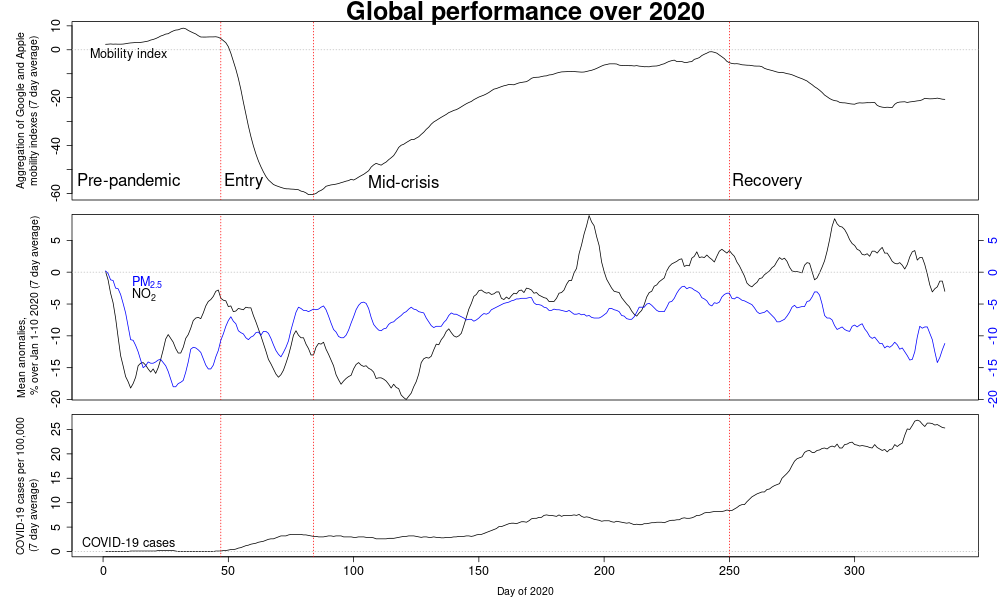
\includegraphics[trim={0 0 15 20},clip,scale=0.45]{Images/LancetPHOverall.png}
\caption{\bf Overview of COVID-19 crisis progression and stages across 507 global cities over 2020. `Entry' begins mid-February 2020 as mobility restrictions are quickly implemented globally, reaching maximum levels in late March, `Mid-crisis'. Early September, the `Recovery' stage corresponds to the end of widespread easing of restrictions and entering a period of localised increases and decreases in stringencies. Seven day rolling average aggregations of Google and Apple mobility indexes (Google mobility workplaces and transit locations and Apple transit and driving map requests) (top), seven day rolling averages of pollution percentage anomalies (PM$_{2.5}$ in blue and NO$_{2}$ in black) over January 1-10, 2020 baseline (middle), and seven day rolling average COVID-19 cases per 100k (bottom).}
 \label{fig:stages}
\end{figure}

\section*{\textcolor{OliveGreen}{Changes in mobility, air pollution, and health outcomes during the COVID observational period}}
\subsection*{Pollution reductions and rebounds}

% script is /home/unimelb.edu.au/knice/git/2024-05-LancetPHPaper2Revision/Rev2Analysis/LPlH-Rev2/PlotFigure7.R
% new script: plot_pollution_as_tsne.R with data from plot_all_pollution.R
\begin{figure}
\centering
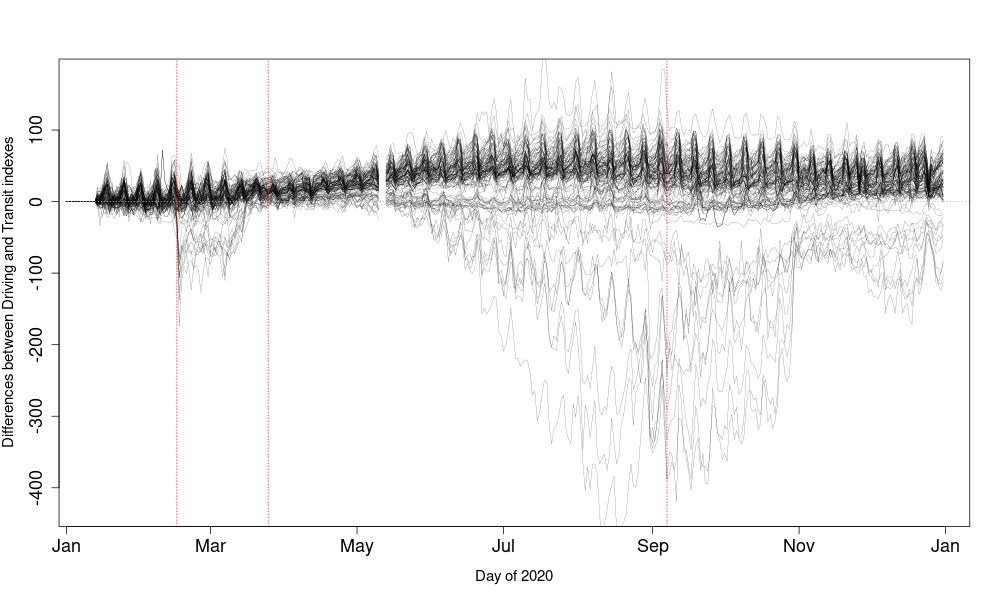
\includegraphics[trim={0 0 0 0},clip,scale=0.4]{Images2/DrivingMinusTransit.png}
\caption{\bf An overview of observed modal shift from public transit to private motor vehicles observed during 2020 for all analysed cities highlighting an increased reliance on private vehicle use over public transit during the course of the COVID-19 pandemic. Values \textgreater 0 indicate a proportional replacement of public transit trips to private vehicles for individual cities in comparison to pre-pandemic conditions.}  
 \label{fig:driv_trans}
\end{figure}


Figure \ref{fig:stages} shows average mobility (Panel 1), anomalies of NO$_{2}$ and PM$_{2.5}$ air pollution levels (Panel 2), and total reported COVID-19 cases (Panel 3) for all measured cities during 2020 across the `Pre-pandemic', `Entry', `Mid-Crisis', and `Recovery' phases of the COVID-19 pandemic. City mobility measures are calculated as seven day rolling average aggregations of Google and Apple mobility indexes (Google mobility workplaces and transit locations and Apple transit and driving map requests) across the 507 cities for which data was available across both city mobility and air pollution (see Box \ref{box:pollution}). Air pollution anomalies are calculated as percentage seven day rolling average differences over a January 1-10, 2020 baseline. COVID-19 cases are calculated as a 7-day rolling average of cases per 100,000 population from Google (2022)\cite{Google2022} (see Box \ref{box:pollution}).

From Figure \ref{fig:stages}, the impact on global city mobility that resulted from the introduction of movement restrictions, including stay-at-home orders, implemented across global cities during the `Entry' phase\cite{hale2021global} of the pandemic can be observed. Although movement restrictions were designed as a public health measure to reduce person-to-person disease transmission, secondary effects were seen related to reductions in global road trauma \cite{ITFRS2023} and significant reductions in mean transport-related NO$_{2}$ and PM$_{2.5}$ levels\cite{zhang2023impact}. Average city mobility declined across cities, reaching a nadir at approximately 45 days post-pandemic onset. This period also coincided with a plateau in global COVID-19 infections (Panel 3) not least because of the public observance of mobility restrictions as well as other non-pharmaceutical interventions implemented up to and including this time\cite{hale2021global}. 

The mean estimated reduction in global NO$_{2}$ and PM$_{2.5}$ levels across observed cities from the beginning of the `Entry' phase until the `Mid-crisis' period were 17.9ppb (3.72\%) and 16.89\si{\micro\gram}/m$^{3}$ (9.35\%), respectively. NO$_{2}$ reductions were likely to have had a substantial effect on reducing health risks for both acute and chronic disease equating to an estimated overall reduction in all-cause mortality risk during this time of 1.5\% (2.2\%-3.0\%), a reduction in cardiovascular mortality risk of 4.1\% (2.6\%-6.0\%), and a reduction in respiratory disease mortality risk of 1.9\% (0.8\%-3.0\%) \cite{Huang19Pollution}. Similarly, reductions in PM$_{2.5}$ levels during this same period equated to estimated reductions in all-cause mortality of 18.9\% (13.2\%-25.0\%)\cite{Yu2020PM2.5}, asthma risk of 46.8\% (18.7\%-65.5\%) and ischaemic heart disease morbidity of 0.25\% (0.2\%-0.3\%)\cite{Xie257}. These effects on relative health risks were continued into the `Mid-crisis' period where reductions in both city mobility and exposure to consequent transport-related air pollution were greatest across regions outside Asia. Using identical means for calculating risk reduction in the Mid-crisis' phase, all-cause mortality estimates related to NO$_{2}$ were consistently around 1.3$\%$ (0.9\%-1.7\%) below baseline, remaining in this range through to the `Recovery' phase (day 250+). Exceptions to this trend were generally found in cities located in the Americas where air pollution-related risk across a range of chronic diseases returned to levels approximating the pre-pandemic baseline or above (see Figure \ref{fig:risks}). These locations have also seen a relative increase in road trauma beyond pre-pandemic levels, which appears associated with uptake of private vehicles in favour of public transport over the same period \cite{ITFRS2023,saladie2023back,DAS20211}. Estimated changes in relative risks associated with air pollution reductions across continents and phases for all-cause mortality, T2 diabetes, asthma and ischaemic heart disease mortality and morbidity for the `Entry', `Mid' and `Recovery' phases of the pandemic are converted from these percentage reductions and presented in Figure \ref{fig:risks} and Table \ref{tab:risks}. 

% script is /home/unimelb.edu.au/knice/git/2022-07-NHMRC_LancetPollution/boxplot/risk_plot3.R (now risk_plot_20250207.R)
\begin{figure}
\centering
\scriptsize{a})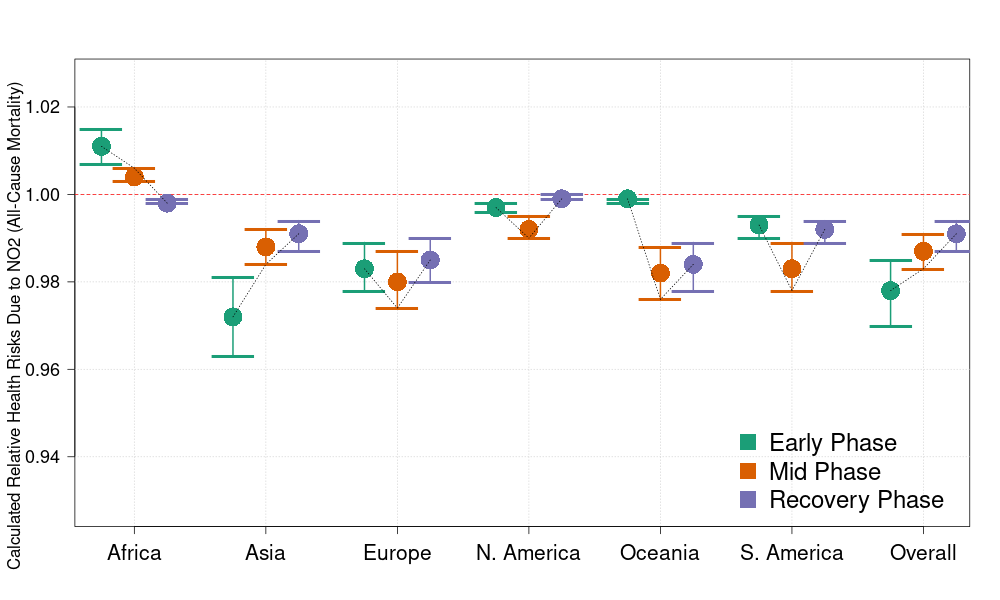
\includegraphics[trim={0 0 25 23},clip,scale=0.23]{Images/no2All_20250207.png}
\scriptsize{b})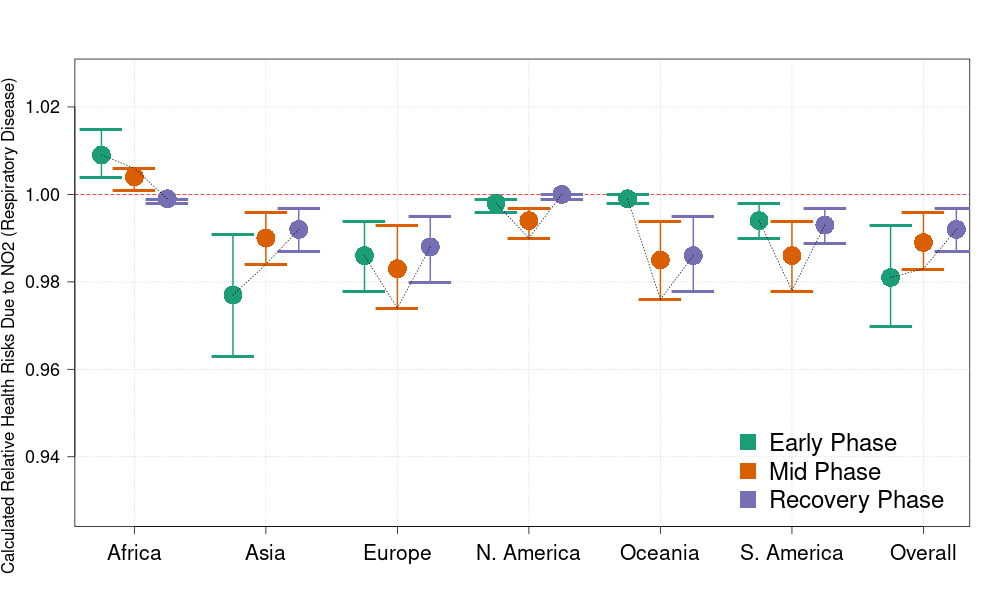
\includegraphics[trim={0 0 25 23},clip,scale=0.23]{Images/no2Res_20250207.png}
\\
\scriptsize{c)}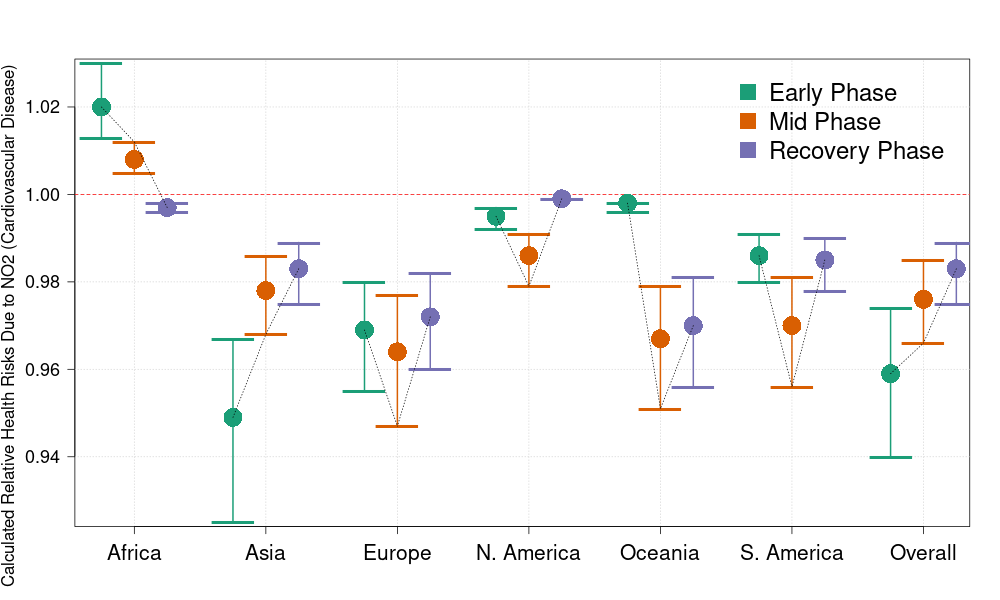
\includegraphics[trim={0 0 25 23},clip,scale=0.23]{Images/no2Car_20250207.png}
\scriptsize{d)}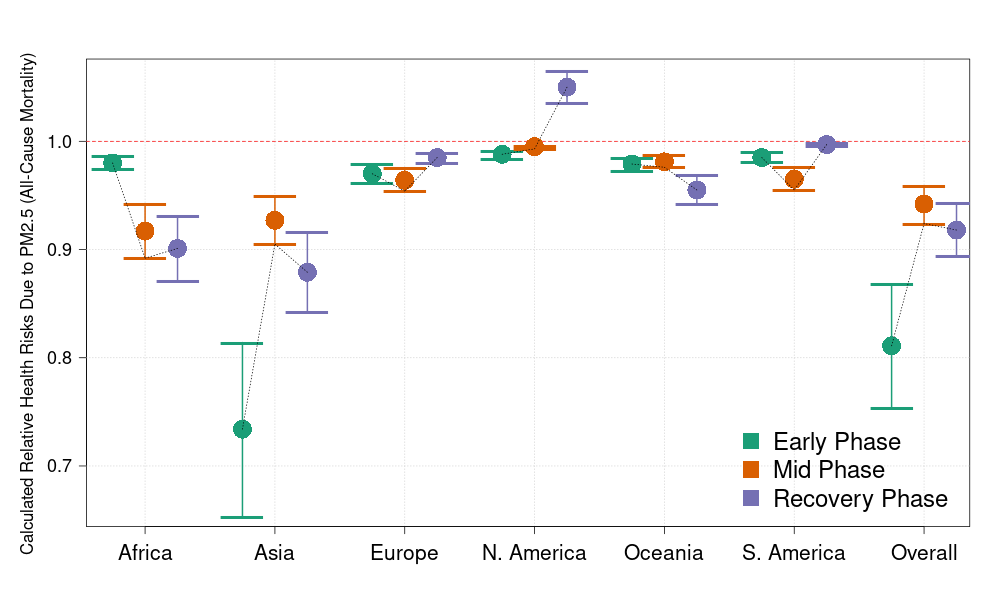
\includegraphics[trim={0 0 25 23},clip,scale=0.23]{Images/pm25All_20250207.png}
\\
\scriptsize{e)}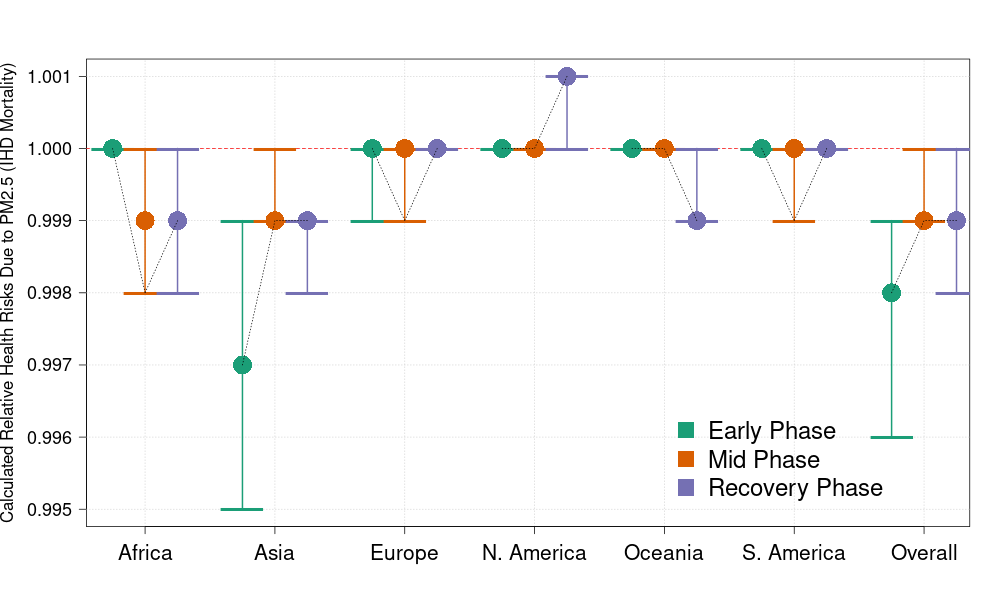
\includegraphics[trim={0 0 25 23},clip,scale=0.23]{Images/pm25Mort_20250207.png}
\scriptsize{f)}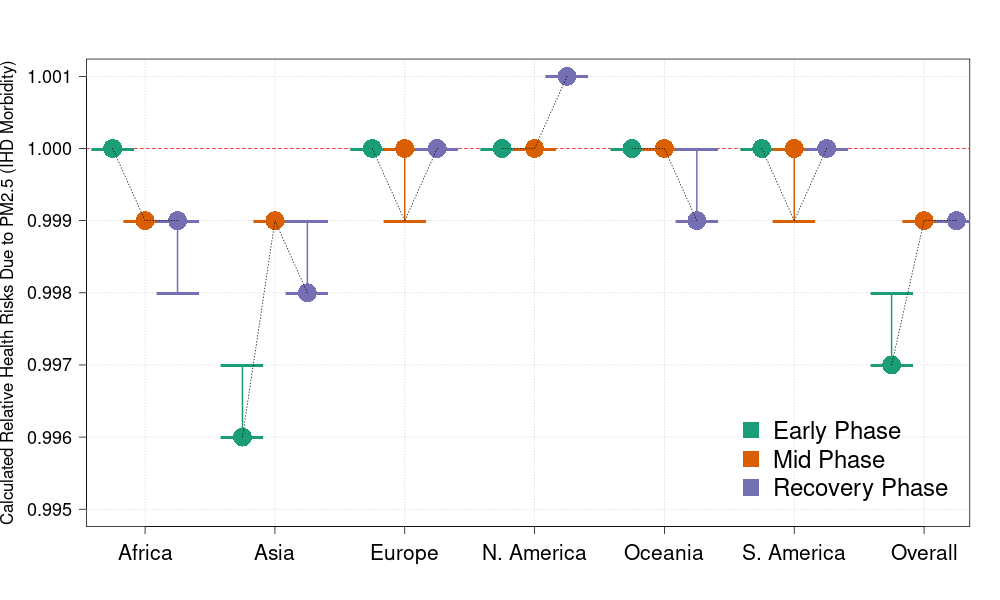
\includegraphics[trim={0 0 25 23},clip,scale=0.23]{Images/pm25Morb_20250207.png}
\\
\scriptsize{g)}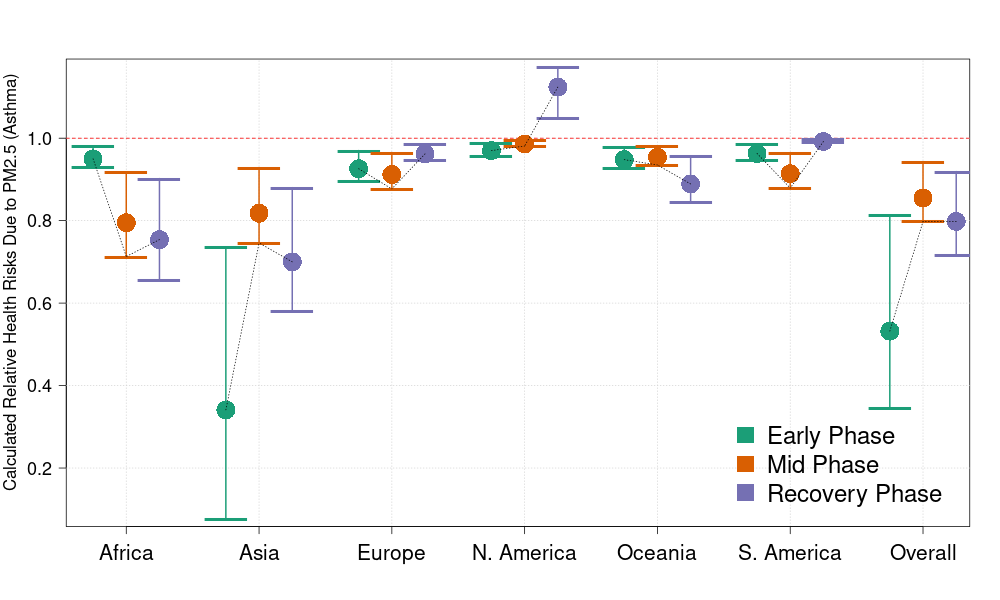
\includegraphics[trim={0 0 25 23},clip,scale=0.23]{Images/pm25Ast_20250207.png}
\caption{\bf Relative health risks (and 95\% confidence interval) associated with air pollution reductions across continents and phases due to 
a) NO$_{2}$ (All-Cause Mortality), 
b) NO$_{2}$ (Respiratory Disease), 
c) NO$_{2}$ (Cardiovascular Disease), 
d) PM$_{2.5}$ (All-Cause Mortality), 
e) PM$_{2.5}$ (IHD Mortality),
f) PM$_{2.5}$ (IHD Morbidity),
g) PM$_{2.5}$ (Asthma). Numbers $>$1 indicate increased health risks.}
 \label{fig:risks}
\end{figure}



\subsection*{Transitions in transport modes during the COVID-19 pandemic}

Alongside private vehicle transport, public transit ridership also declined by up to 90\% in the pandemic's `Entry' phase\cite{TransitCovid_Gkiotsalitis}. However, as city mobility restrictions eased in response to declining rates of COVID-19 transmission and populations began re-engaging with workplaces and social settings, citizens were faced with new factors that influenced their transportation choices including the risk of infection through the use of mass transit\cite{BECKTransit}. Figure \ref{fig:driv_trans} shows how these concerns contributed to a global shift away from public transport toward private vehicle use with values \textgreater 0 indicating a proportional modal shift away from public transit and toward private vehicle use. This trend across the vast majority of cities was most evident during July and August 2020, but continued until early 2021 with many cities later implementing incentive programs to boost public transit ridership \cite{dai2021improving}. Global trends are summarised in Table \ref{tab:driving}.

\begin{table}
\caption{Changes in private vehicle use across continents and phases in percentages over the baseline. Negative numbers indicate a reduction of private vehicle use.}
\begin{tabular}{ |l|l|l|l| }
\hline
\textbf{Region} & \textbf{Early Phase} & \textbf{Mid Phase} & \textbf{Recovery Phase}  \\ 
\hline
%\multicolumn{4}{ |c| }{Driving Changes by Contient and Phase} \\
%\hline \hline
%Region & Early Phase & Mid Phase & Recovery Phase  \\ \hline
Africa         & \cellcolor{red!12}12.87 & \cellcolor{blue!15}-48.88 & \cellcolor{blue!10}-2.78  \\ \hline
Asia           & \cellcolor{red!15}21.29 & \cellcolor{blue!10}-15.69 & \cellcolor{red!10} 7.16  \\ \hline
Europe         & \cellcolor{red!13}18.07 & \cellcolor{blue!20}-78.44 & \cellcolor{red!25} 45.25  \\ \hline
North America  & \cellcolor{red!12}13.49 & \cellcolor{blue!16}-54.71 & \cellcolor{red!10}4.07  \\ \hline
Oceania        &  \cellcolor{red!10}9.51 & \cellcolor{blue!15}-43.18 & \cellcolor{blue!10}-5.97  \\ \hline
South America  & \cellcolor{red!12}15.67 & \cellcolor{blue!18}-67.23 & \cellcolor{red!10}9.04  \\ \hline
\end{tabular}\label{tab:driving}
\end{table}

Examining Panel 2 of Figure \ref{fig:stages}, it is clear that the timing of the increase in private vehicle transport in mid-2020 coincided with a significant rebound of NO$_{2}$ and PM$_{2.5}$ back to levels that would be typically expected under `normal' conditions (adjusting for weather, and trends in seasonality, distinct topography, urban morphology, climate, and atmospheric conditions of each city\cite{Wijnands2022}). This rebound was particularly pronounced for NO$_{2}$, which consistently exceeded normal pre-pandemic levels across cities in the latter part of 2020.

However, despite the global trend of transitioning from public transit to private motor vehicle use\cite{fernando2023shaping}, our results reveal that the extent of this shift was not uniform across all city types. Mode shift  was more pronounced in cities recognised as being largely designed for motor vehicles\cite{Thompson2020} represented in grid areas A3 to A5 and B4 to B6 of Figure \ref{fig:tSNE}. The effect of this on transport-related pollution in the form of PM$_{2.5}$ and NO$_{2}$ is highlighted in Figures \ref{fig:Heatmap250PM}a and \ref{fig:Heatmap250NO2}b, presenting mean anomalies for these pollutants for cities located in each grid reference tile, respectively. To recall, cities in these grid locations typically demonstrate regular (e.g., quadrilateral), medium-sized blocks with medium to comparatively low levels of public transit.

% new script
% /home/unimelb.edu.au/knice/git/2024-05-LancetPHPaper2Revision/Rev2Analysis/LPlH-Rev2/Pollution/plot_pollution_as_tsne.R
\begin{figure}
\centering
%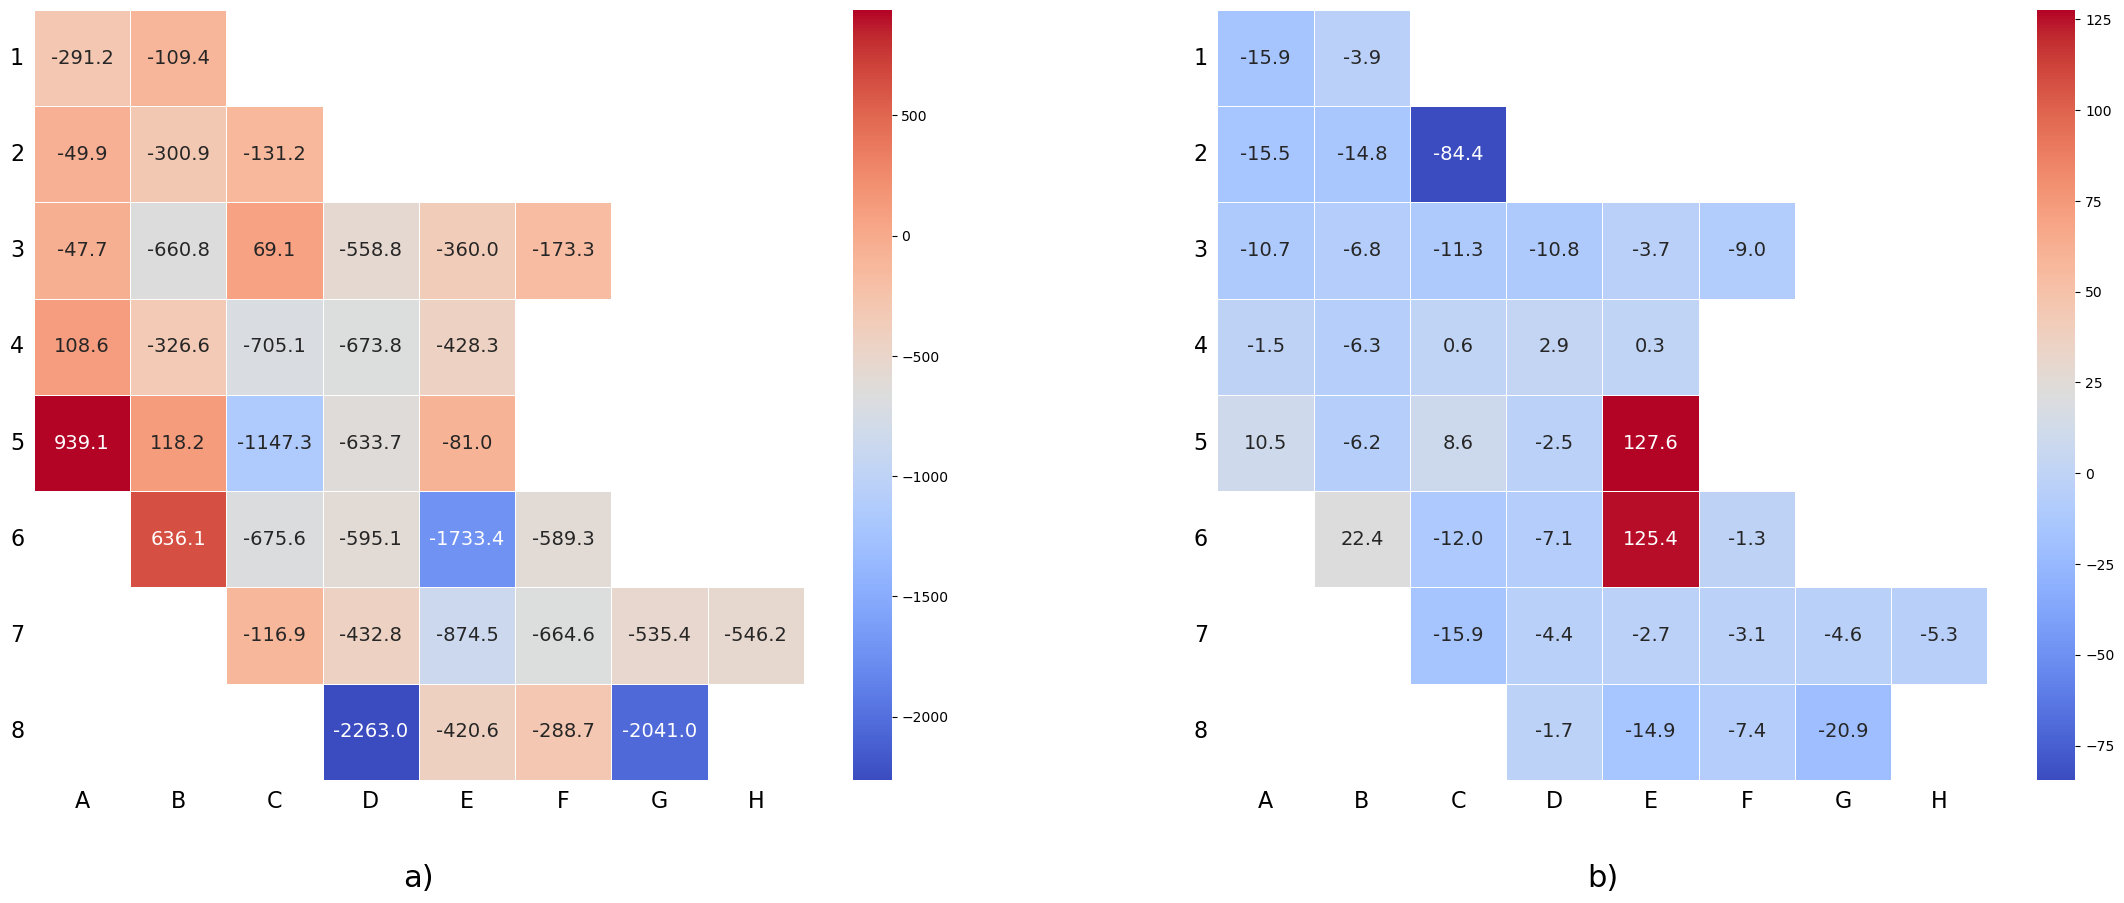
\includegraphics[trim={0 0 0 0},clip,scale=0.25]{Images/pm25Anomaly250_no2Reduction7Ave7Ave250.png}
a) 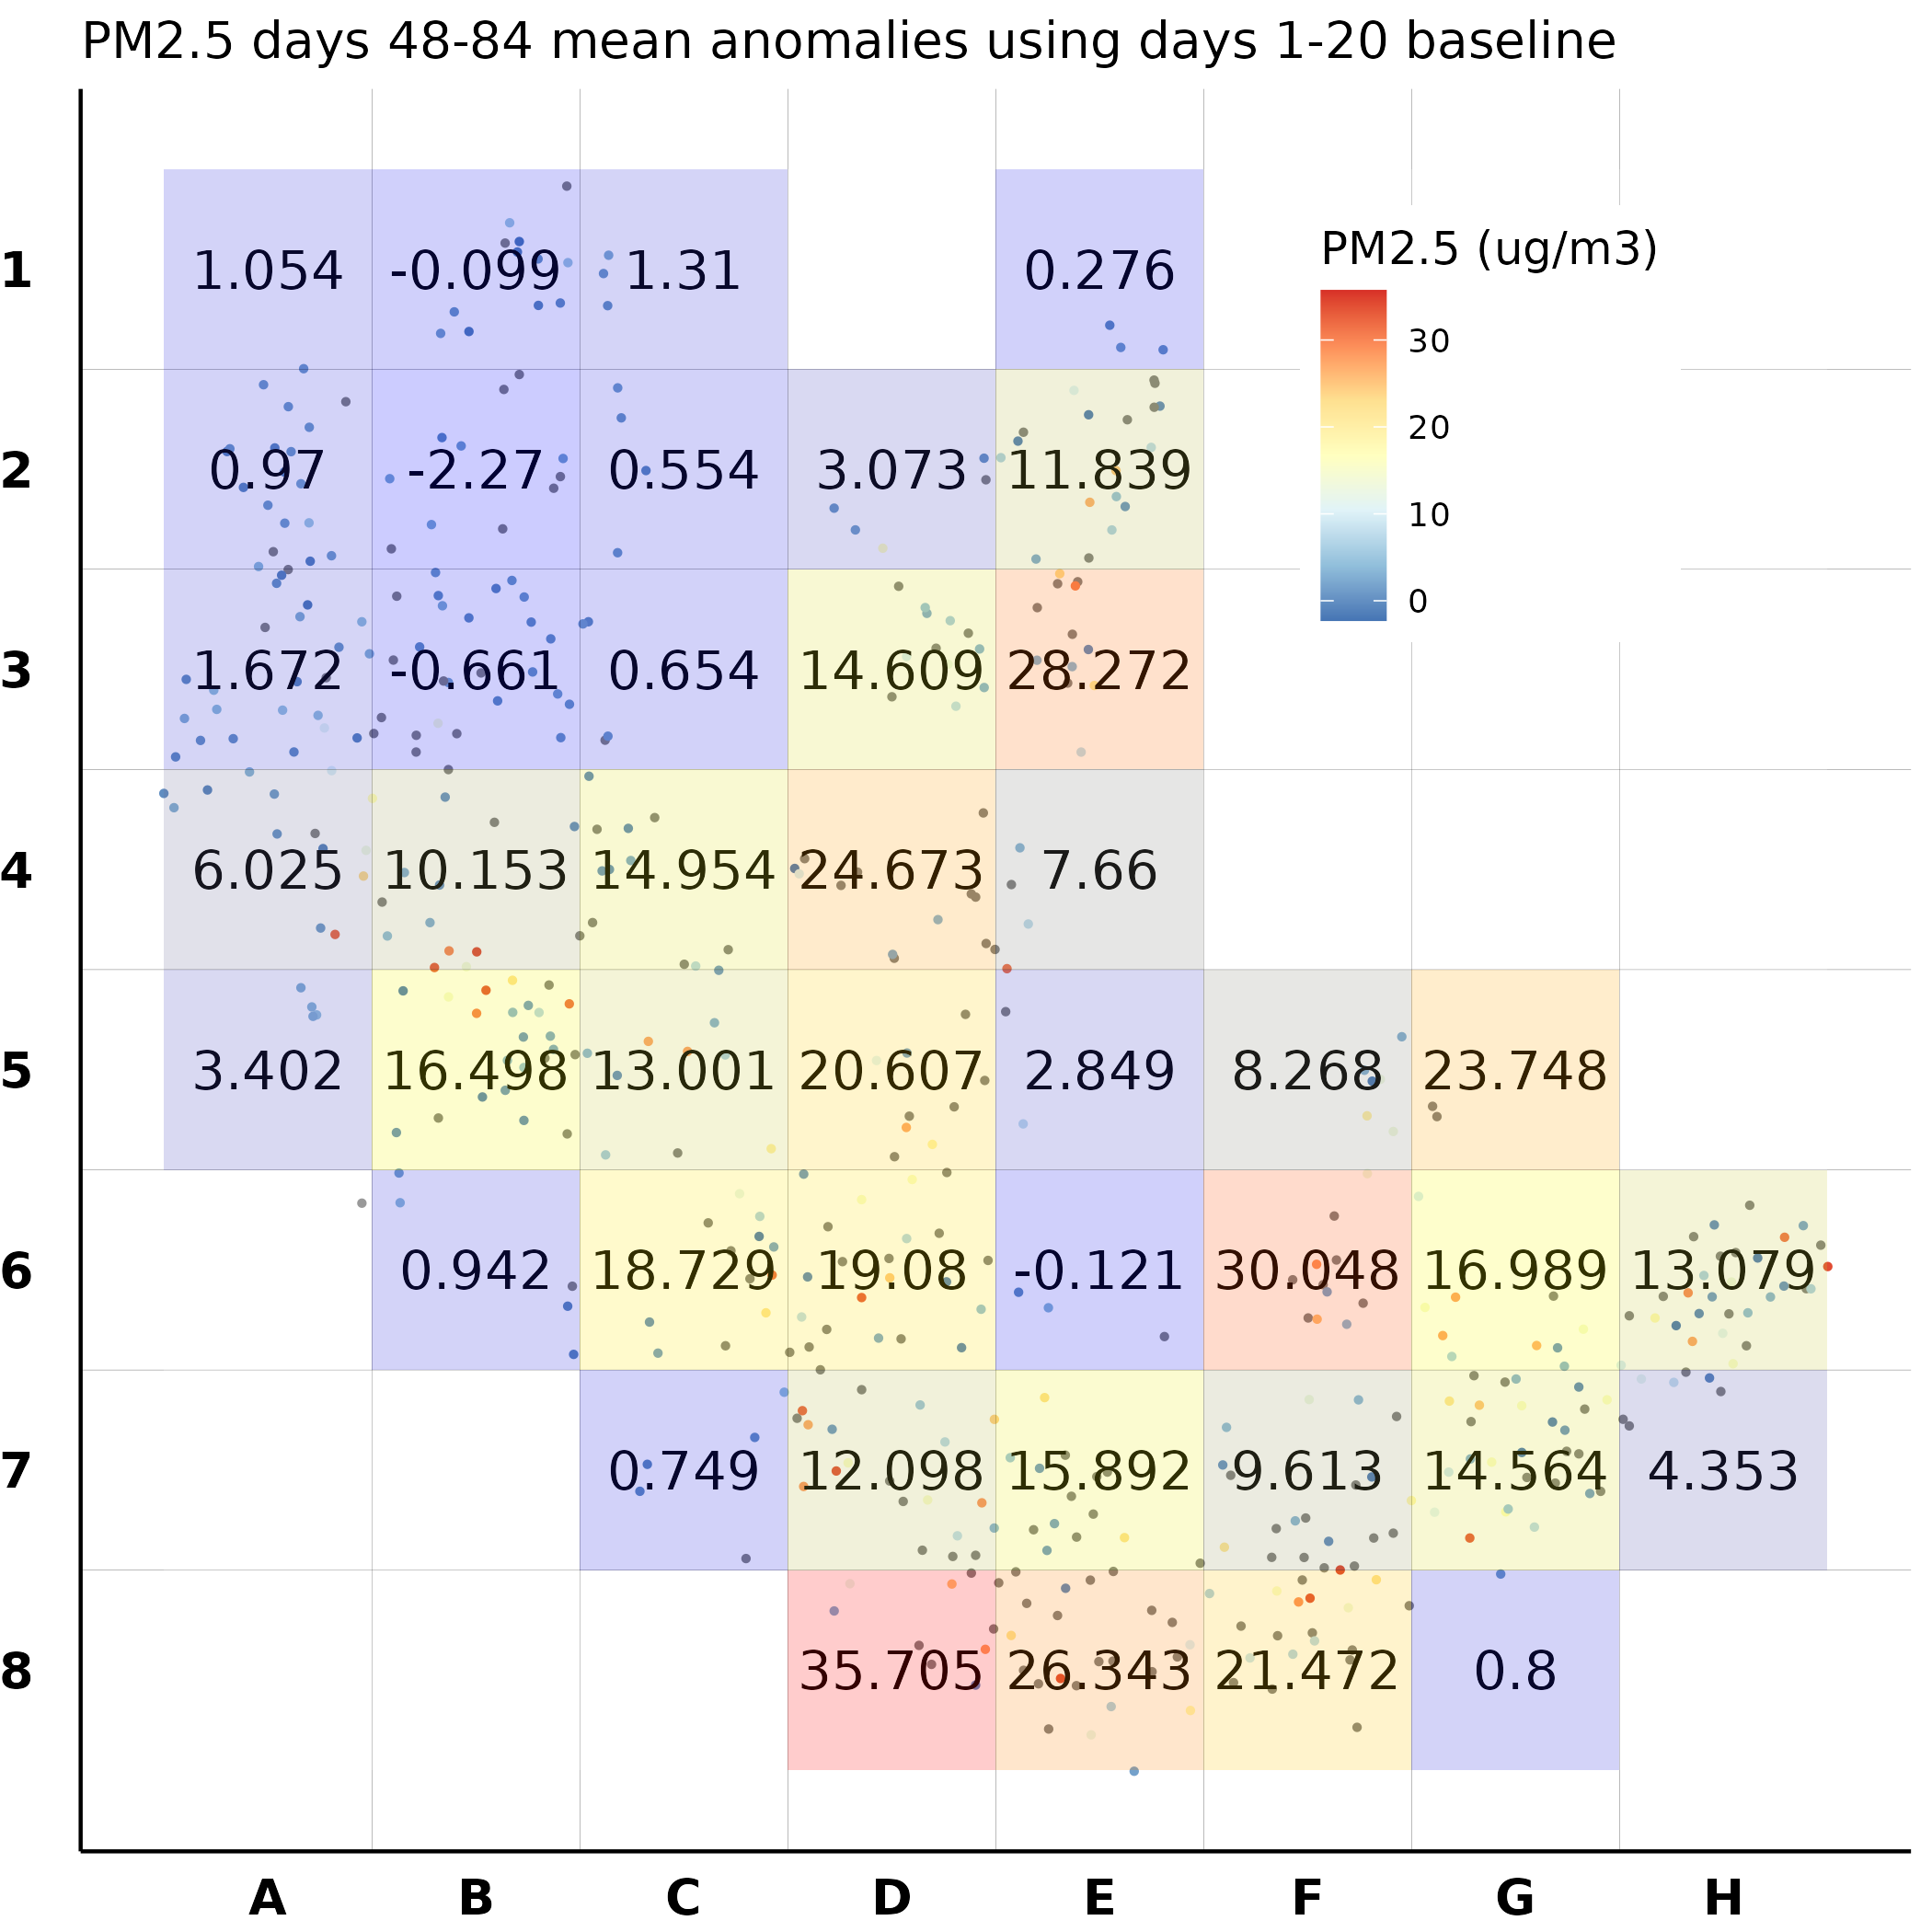
\includegraphics[trim={0 0 0 0},clip,scale=0.43]{Images/City_Types_Dimension_chessboard_pm25anomalyDiff20.png}
b) 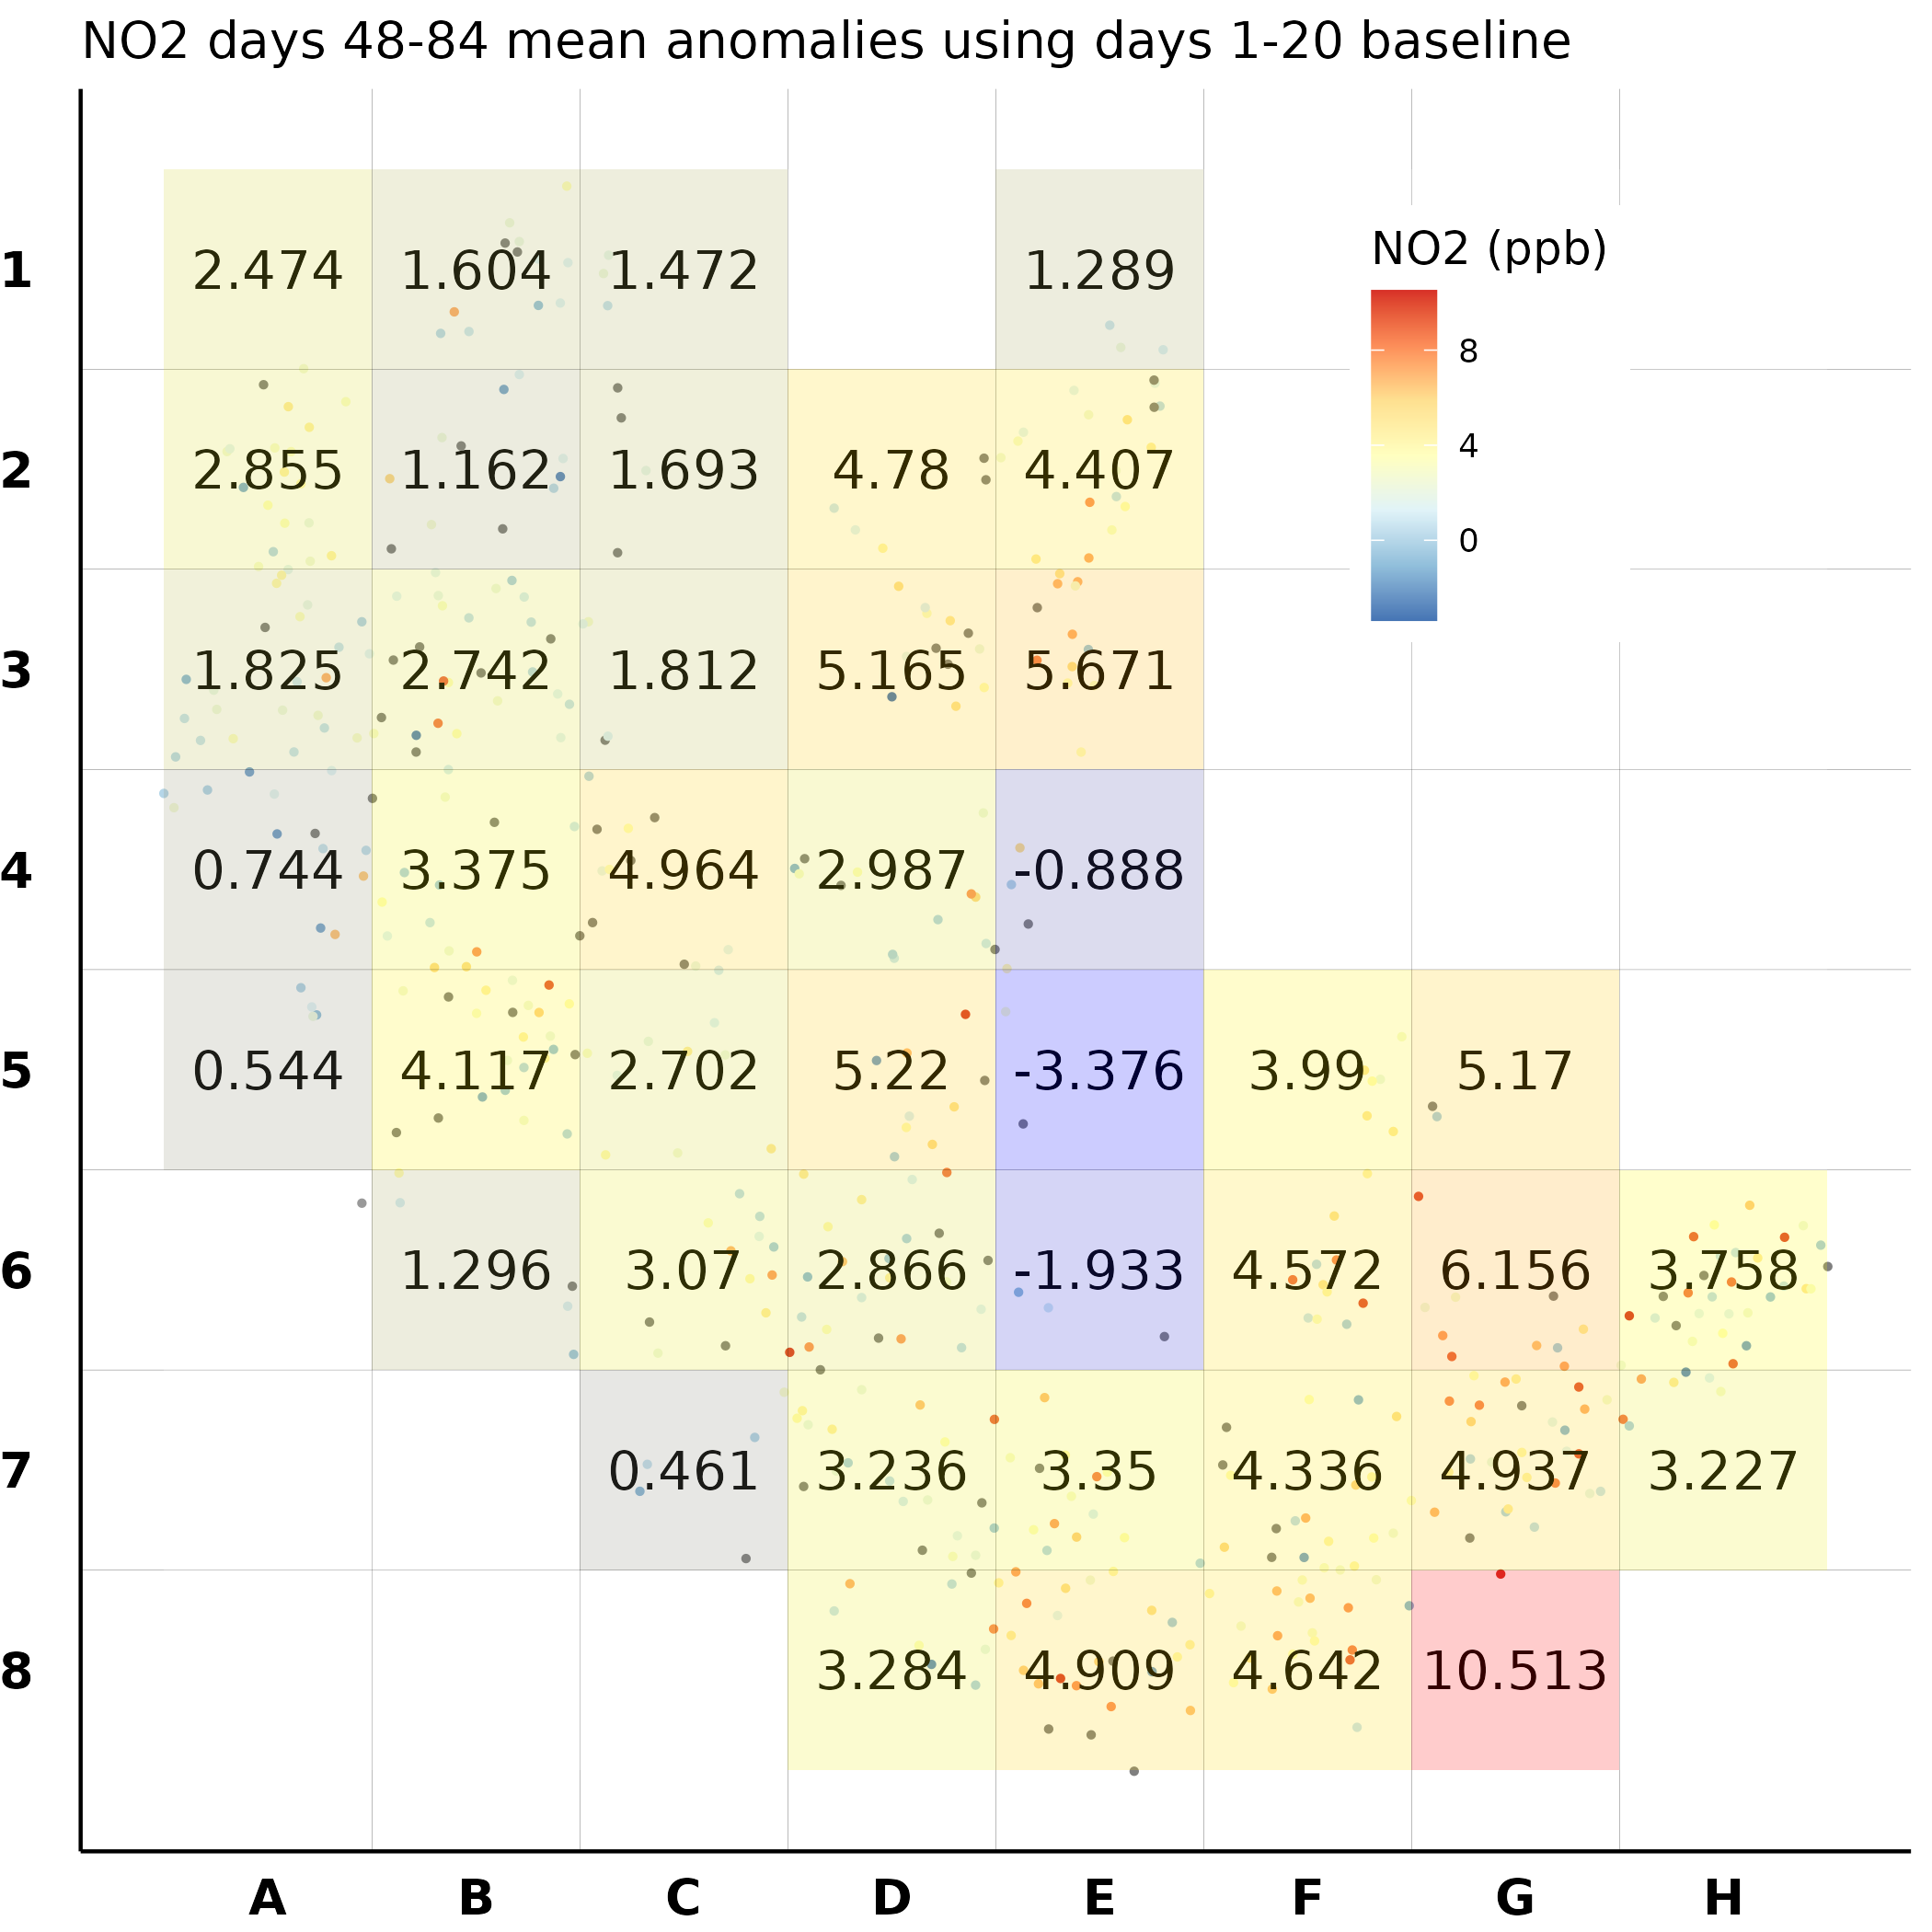
\includegraphics[trim={0 0 0 0},clip,scale=0.43]{Images/City_Types_Dimension_chessboard_no2anomalyDiff20.png}
\caption{\bf Mean anomalies of a) PM$_{2.5}$ (\si{\micro\gram}/m$^{3}$) and b) NO$_{2}$ (ppb) across the period of days 84 to 250 in 2020 for cities in each grid reference tile and underlying values for each city (see Figure \ref{fig:tSNE}).}  
 \label{fig:Heatmap250NO2}\label{fig:Heatmap250PM}
\end{figure}

\subsection*{City designs that saw transitions to private motor vehicle use}

The characteristic design of cities designed to promote the egress of motor vehicles is that they have planned, regular block layouts (for instance, quadrilateral block patterns) and have blocks of medium-size in comparison to other global cities\cite{Thompson2020}. Such vehicle-centric city designs are predominantly found in countries including the United States, Australia, Canada, New Zealand, and Argentina, which have seen rapid urban expansion in the late 19th and early 20th centuries. During the COVID-19 pandemic's `Mid Crisis' and `Recovery' phases as defined here, cities optimised for private vehicle transport afforded citizens a choice between public transit and private vehicle use. Given the public's fear of potential infectious disease transmission on public transit\cite{fernando2023shaping}, citizens who had the option to avoid public transit in favour of private vehicles did so en-mass. In these cities, public transit ridership did not rebound to pre-pandemic levels within the observation period. 


\begin{figure}
     \centering
    % \begin{subfigure}[b]{0.9\textwidth}
        % \centering
       \scriptsize a)~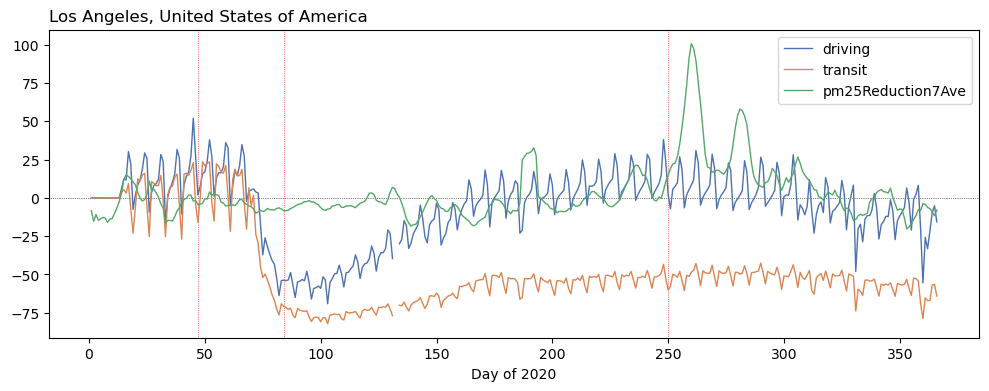
\includegraphics[width=\textwidth,trim={0 37 0 0},clip]{Images/LA_Drive_trans_pm25.png}
        % \caption{Los Angeles, United States of America}
         \label{fig:LosAngeles}
    % \end{subfigure}
     %\hfill
    % \begin{subfigure}[b]{0.9\textwidth}
       %  \centering
         b)~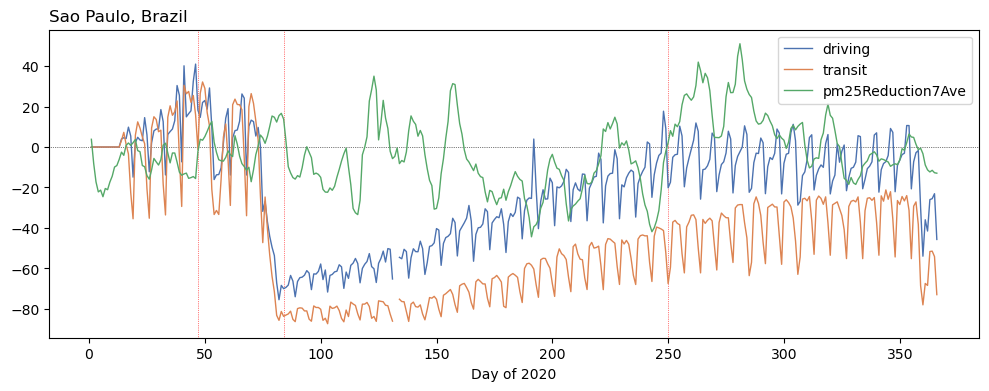
\includegraphics[width=\textwidth,trim={0 37 0 0},clip]{Images/SaoPaulo_Drive_trans_pm25.png}
         %\caption{Sao Paulo, Brazil}
         \label{fig:SaoPaulo}
    % \end{subfigure}
     %\hfill
    % \begin{subfigure}[b]{0.9\textwidth}
       %  \centering
         c)~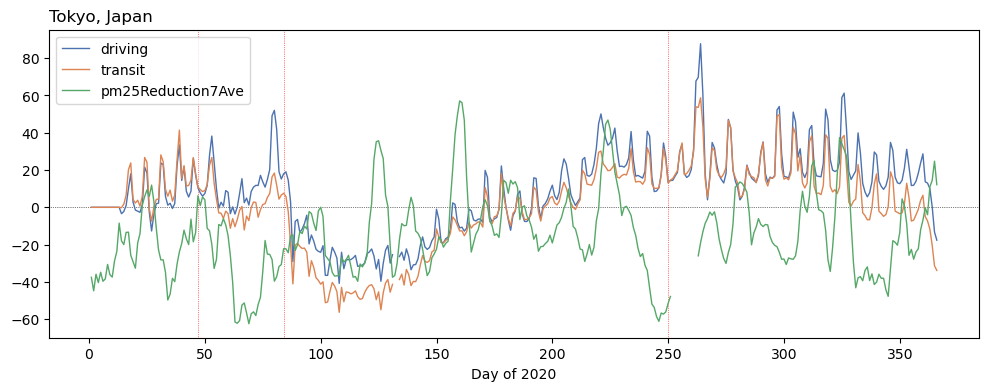
\includegraphics[width=\textwidth]{Images/Tokyo_Drive_trans_pm25.png}
        % \caption{Tokyo, Japan}
         \label{fig:Tokyo}
    % \end{subfigure}
        \caption{\bf An overview of the shifts in transportation mode preferences (daily Apple Mobility indexes for driving and transit modes in red and blue) and PM$_{2.5}$ anomalies over 2020 (7 day rolling averages of PM$_{2.5}$ anomalies in green) for three example cities a) Los Angeles, United States of America, b) S\~ao Paulo, Brazil and c) Tokyo, Japan. Highlighted is an increased reliance during the course of the COVID-19 pandemic on private vehicle use over public transit in Los Angeles and S\~ao Paulo while minimal changes in transport mode share between public transit and private motor vehicles in Tokyo. Extremes in PM$_{2.5}$ readings in Los Angeles may have also been exacerbated by summer wildfires on select days.}
        \label{fig:three_graphs_Driv_trans}
\end{figure}

For example, an archetypal city demonstrating a regular, car-based network is Los Angeles, USA. Figure \ref{fig:three_graphs_Driv_trans}a shows the relative change in mode share between public transit and private vehicles for Los Angeles from a pre-pandemic baseline during 2020 in addition to showing anomalies from expected levels of PM$_{2.5}$ pollution over the same period. Notable is that while observed patterns of city mobility for Los Angeles' residents largely returned to normal in the second half of 2020, public transit remained well below baseline. Importantly, the trade-off between public transit and private vehicle use during the `Recovery' phase was also associated with a peak in PM$_{2.5}$ pollution. While a proportion of this pollution peak on select days was likely attributable to active wildfires, this pattern of results was consistently observed across similarly organised cities in North America and other cities whose designs located them in grid areas C1 to C3 and B1 to B3 of Figure \ref{fig:tSNE} representing those with predominantly private car-based transport systems. In S\~ao Paulo, Brazil (Figure \ref{fig:three_graphs_Driv_trans}b), similar mobility shifts are seen. However, while Los Angeles' transit rates stagnated at low levels across the remainder of 2020, transit usage in S\~ao Paulo began recovery toward baseline levels, although at a much slower rate than the earlier transition to private vehicle use.

For the average of both North and South American locations, the combination of increased air pollution levels, disease risk, and increased private vehicle transport also coincided with the highest reported per-capita COVID-19 cases, globally (see Figure \ref{fig:covidCases7Ave})\footnote{https://github.com/GoogleCloudPlatform/covid-19-open-data/blob/main/docs/table-epidemiology.md}. It is not possible to draw direct causal relationships between these data, except perhaps to the extent that infection rates increased from already comparatively high global rates - especially in North America - once levels of mobility began increasing again. This pattern was in contrast to some locations (e.g., in Asia and Oceania) that had maintained comparatively low levels of COVID-19 in the mid-pandemic phase. Of course, because these data relate to `reported' cases, they are also subject to some interpretation given differences in testing and reporting regimes between regions.

\begin{figure}
\centering

% being replaced by 
% /home/unimelb.edu.au/knice/git/2021-08-COVIDPollutionPaper/Analysis/plot_covid_cases_fig11.R
% data from combinedData_Intep_COVIDCASES.csv by LancetCombineDatasetsCovidCases.java taken from COVID-19-open-data
\includegraphics[trim={0 0 0 0},clip,scale=0.45]%{Images/Average_Covid_Cases_Plot.png}
{Images/covid_cases_continents.png}
%}
\caption{\bf Mean reported COVID-19 cases per 100,000 population across continents in 2020 for the Early, Mid-Crisis, and Recovery pandemic phases with error bars representing standard deviations across countries within regions.}  
 \label{fig:covidCases7Ave}
\end{figure}

For example, Figure \ref{fig:three_graphs_Driv_trans}c demonstrates that the rebound in city mobility in the second half of 2020 in the city of Tokyo, Japan did not result in a sustained modal transfer between public transit and private vehicles. Similarly, neither did this rebound coincide with peaks in transport-related air pollution nor widespread COVID-19 infections. This pattern of results was observed across Japanese cities, which are peculiar on the world stage in that they combine very dense road networks and very small blocks with high levels of public transit alongside policies that restrict on-street vehicle parking\cite{clements2019socialising}. Japanese cities' combination of city design and public policy shifts responsibility for parking provision onto individual vehicle owners rather than to local government, tipping the scales of transport choice away from private means and disincentivising car ownership. Therefore, while car-centric city designs and associated policies in some countries afforded populations transport mode choice and a shift toward private vehicle use when concerns regarding infectious disease transmission on public transit were high, Japanese cities and their supporting policies constrained citizens' capacity to shift away from public transport quickly even if they wanted to, resulting in a relative return to normal in the pandemic's `Recovery' phase.


\section*{\textcolor{OliveGreen}{The influence of city design and transport mode choice on health outcomes}}
\subsection*{Which city types had greater resilience against the adverse health effects of the crises?}

The results presented here indicate that city designs afforded populations across the world different tools to adapt and deal with the threat posed by COVID-19 as the crisis unfolded, and their responses also had both beneficial and harmful consequences during progressive phases. If we consider resilience as the "ability of a system, community or society exposed to hazards to resist, absorb, accommodate to and recover from the effects of a hazard in a timely and efficient manner, including through the preservation and restoration of its essential basic structures and functions" \cite{unisdr2009terminology}, this led some city types to demonstrate greater defence against public health threats than others.

First of all, there appears to have been a demonstrable reduction in air pollution and related disease risk within cities where mobility restrictions were enforced by governments seeking to reduce person-to-person interaction and therefore, infectious disease spread. Despite the threat posed by COVID-19 on an unvaccinated population at the time, these secondary benefits were realised most acutely in the `Entry' and `Mid-crisis' phases of the pandemic when city mobility was most greatly reduced. Further, while no globally consistent data sources on road trauma at the daily, city level are available, evidence suggests that this period also saw a considerable reduction in road trauma across the world in both raw numbers of deaths and injuries \cite{saladie2023back,ITFRS2022,ITFRS2023,GBDStudy}. As described below, however, this effect was short-lived.

\subsection*{Risk reductions were short-term in most locations while others maintained greater resilience}
Unfortunately, many of the early benefits accrued from reductions in air pollution were not sustained, even until the end of 2020. Further, with the desire to rebound to prior levels of economic activity and mobility, many cities designed for private, car-based transport and where private vehicles have been favoured over public or active transit options\cite{DAS20211}, also rebounded to levels of air pollution and associated chronic disease risk that were equal to, if not exceeding, pre-pandemic levels; some of the few public health benefits of the pandemic era were lost. Added to this are widely observed post-pandemic rebounds in global road trauma (see Figure \ref{fig:GBD}). For example, in its 2023 report, the International Traffic Safety Data and Analysis Group (IRTAD), which described 2020 and 2021 as `exceptional years' in terms of reductions in road trauma among its member nations, laments that fatalities in many countries have now returned beyond their pre-pandemic levels. In particular, it highlights that that countries including the United States (27\%), New Zealand (22\%), Israel (21\%) and Costa Rica (20\%) appear to be witnessing even higher rates of road trauma than were experienced a decade prior. This pattern contrasts with significant road fatality declines in countries such as Japan (-39\%), Lithuania (-60\%), Korea (-50\%), Poland (-47\%), Greece (-35\%), Belgium (-34.7\%), Slovenia (-34\%), and Austria (-30\%) \cite{ITFRS2022,ITFRS2023}. Differences in post-pandemic road trauma patterns observed between regions are consistent with what might be expected given the dominant city and transport types housed within each country and explored within this study.

\begin{figure}
\centering

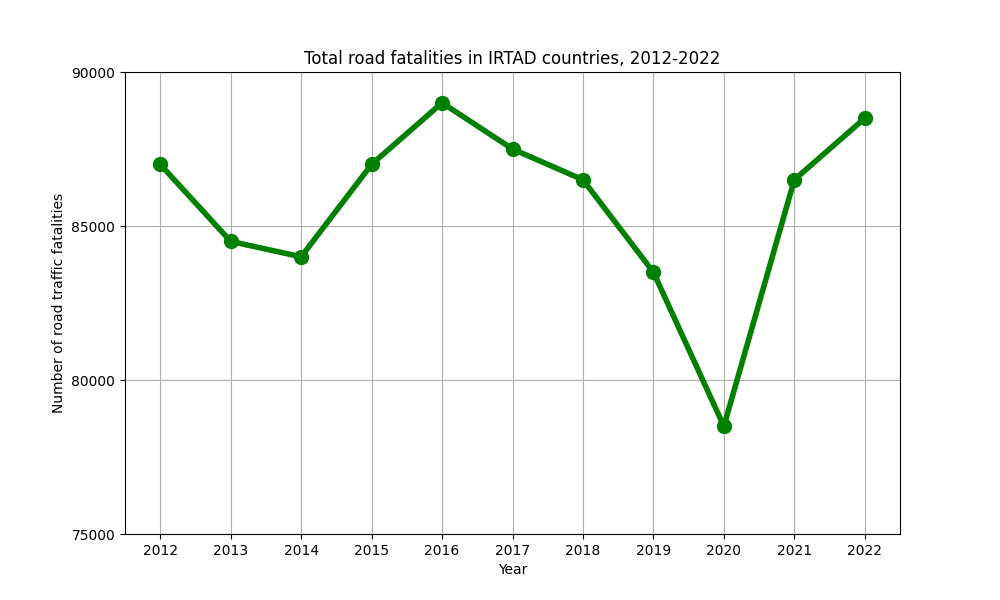
\includegraphics[trim={0 0 0 0},clip,scale=0.5]{Images/Recreated.png}
%}
\caption{\bf Changes in total road traffic fatalities among the 43 member countries contributing to the International Traffic Safety Data and Analysis Group (IRTAD) showing a post-pandemic (2020-2021) rebound (figure adapted from \cite{ITFRS2023}).}  
 \label{fig:GBD}
\end{figure}



\subsection*{Optimal city types for health vary by crisis and stage of the crisis}

The results above demonstrate that optimal city types for health are not static, but change over time given the dynamic nature of health crises and concerns. This should come as little surprise given the role of cities and shared urban infrastructure in historic public health challenges. However, the performance of cities and their role in producing or preventing disease has previously tended to be considered over a period of centuries, decades or multiple years. Here, we demonstrate that optimal designs for health can change amid crises that unfold over weeks and months.

Beyond infrastructure and design, we also acknowledge that embedded transport `cultures' \cite{PATERSON_2000} can influence whether rapid changes to transport mode share `stick' or not. This is a direction for future research. For example, that so many locations around the world experienced substantial reductions in pollution, road trauma, and associated chronic disease health risks during 2020 and 2021 appears to have been insufficient incentive for more societies to seek a more permanent transition away from transport modes that contribute to such risks. In fact, in many locations, car culture has not only been resilient to change but has strengthened, especially where city design has facilitated it and even where strategy has attempted to prevent it or at least lock-in benefits of alternative, active and sustainable transport modes\cite{hunter_city_2024}. In this sense, it might be reasonable to consider some instances of resilience - i.e., \textit{`preservation and restoration of ... essential basic structures and functions'} - as counter-productive to progress on overall planetary and/or population health. This is pertinent when we consider that more than half of the world's greenhouse gas (GHG) emissions have arisen in the period following the United Nations Framework Convention for Climate Change in 1992\cite{bashmakov2022climate}, with road transport one of the most significant contributors. The societal challenge to subvert some elements of resilient city designs in efforts to transition to net zero by 2050\cite{lynskey2020moving} is considerable.

\subsection*{Conclusions}

Cities generate social and economic benefits for individuals and societies, alike. Large cities generate significant interaction, trade, creativity, and promote efficiency by placing people and resources in close proximity to one another \cite{bettencourt2013origins}. Because of this, they are also places where the majority of the world's population choose to live. However, the design of cities also produce and facilitate unwanted and persistent problems; among them, disease, pollution, and injury. This observational study has demonstrated that such disadvantages are not a \textit{fait accompli} but more-or-less a consequence of city design. It highlights that city design affects the extent to which these negative aspects manifest, especially amid crises. It also suggests the prestige and (ill-)health experienced by citizens in even the greatest or `healthiest' of cities may be ephemeral. Times, circumstances, environments, and phases of unfolding crises can appear rapidly, exposing citizens and societies to new risks and public health challenges, some of which are based on responses to those same crises (\cite{hunter_city_2024, garcia_city_2024}. Of perhaps greatest importance given the evidence presented here is that city designs enable dynamism, building in transport and urban systems that enable rapid adaptation when needs arise.



\section*{Contributors}\label{sec:credit}
KAN and JT conceived and designed the study and wrote the manuscript. KAN collected the mobility and pollution data and KAN and JT analysed the data. HZ and SS performed data analysis and helped develop the methods. All authors contributed to developing, writing and editing the manuscript and interpreting the findings.

\section*{Declaration of interests}\label{sec:dec}
We declare no competing interests.


\bibliography{bibtext.bib}
\bibliographystyle{elsarticle-num} 
%\bibliography{bib}
%\begin{thebibliography}{1}
\expandafter\ifx\csname url\endcsname\relax
  \def\url#1{\texttt{#1}}\fi
\expandafter\ifx\csname urlprefix\endcsname\relax\def\urlprefix{URL }\fi
\expandafter\ifx\csname href\endcsname\relax
  \def\href#1#2{#2} \def\path#1{#1}\fi

%\end{thebibliography}


\section{Supplementary Material}
\beginsupplement

\begin{table}
\caption{Relative health risks (and 95\% confidence interval) associated with air pollution reductions across continents and phases. Numbers $>$1 indicate increased health risks.}
\scalebox{0.9}{\begin{tabular}{ |l|l|l|l| }
\hline
\textbf{Region} & \textbf{Early Phase} & \textbf{Mid Phase} & \textbf{Recovery Phase}  \\ \hline\multicolumn{4}{ |l| }{Mean NO$_{2}$ anomaly(ppb) : Estimated Relative Health Risks Due to NO$_{2}$ (All-Cause Mortality) (Lower -- Upper bound)} \\
\hline 
%Region & Early Phase & Mid Phase & Recovery Phase  \\ \hline
Africa & 1.86 : 1.011 (1.007 -- 1.015) & 0.72 : 1.004 (1.003 -- 1.006) & -0.28 : 0.998 (0.999 -- 0.998)
 \\ \hline
Asia & -4.66 : 0.972 (0.981 -- 0.963) & -2 : 0.988 (0.992 -- 0.984) & -1.58 : 0.991 (0.994 -- 0.987)
 \\ \hline
Europe & -2.81 : 0.983 (0.989 -- 0.978) & -3.31 : 0.98 (0.987 -- 0.974) & -2.5 : 0.985 (0.99 -- 0.98)
 \\ \hline
North America & -0.48 : 0.997 (0.998 -- 0.996) & -1.29 : 0.992 (0.995 -- 0.99) & -0.09 : 0.999 (1 -- 0.999)
 \\ \hline
Oceania & -0.22 : 0.999 (0.999 -- 0.998) & -3.04 : 0.982 (0.988 -- 0.976) & -2.72 : 0.984 (0.989 -- 0.978)
 \\ \hline
South America & -1.23 : 0.993 (0.995 -- 0.99) & -2.77 : 0.983 (0.989 -- 0.978) & -1.39 : 0.992 (0.994 -- 0.989)
 \\ \hline
Overall & -3.72 : 0.978 (0.985 -- 0.97) & -2.15 : 0.987 (0.991 -- 0.983) & -1.58 : 0.991 (0.994 -- 0.987)
 \\ \hline
\multicolumn{4}{ |l| }{Mean NO$_{2}$ anomaly(ppb) : Estimated Relative Health Risks Due to NO$_{2}$ (Respiratory Disease) (Lower -- Upper bound)} \\
\hline 
%Region & Early Phase & Mid Phase & Recovery Phase  \\ \hline
Africa & 1.86 : 1.009 (1.004 -- 1.015) & 0.72 : 1.004 (1.001 -- 1.006) & -0.28 : 0.999 (0.999 -- 0.998)
 \\ \hline
Asia & -4.66 : 0.977 (0.991 -- 0.963) & -2 : 0.99 (0.996 -- 0.984) & -1.58 : 0.992 (0.997 -- 0.987)
 \\ \hline
Europe & -2.81 : 0.986 (0.994 -- 0.978) & -3.31 : 0.983 (0.993 -- 0.974) & -2.5 : 0.988 (0.995 -- 0.98)
 \\ \hline
North America & -0.48 : 0.998 (0.999 -- 0.996) & -1.29 : 0.994 (0.997 -- 0.99) & -0.09 : 1 (1 -- 0.999)
 \\ \hline
Oceania & -0.22 : 0.999 (1 -- 0.998) & -3.04 : 0.985 (0.994 -- 0.976) & -2.72 : 0.986 (0.995 -- 0.978)
 \\ \hline
South America & -1.23 : 0.994 (0.998 -- 0.99) & -2.77 : 0.986 (0.994 -- 0.978) & -1.39 : 0.993 (0.997 -- 0.989)
 \\ \hline
Overall & -3.72 : 0.981 (0.993 -- 0.97) & -2.15 : 0.989 (0.996 -- 0.983) & -1.58 : 0.992 (0.997 -- 0.987)
 \\ \hline
\multicolumn{4}{ |l| }{Mean NO$_{2}$ anomaly(ppb) : Estimated Relative Health Risks Due to NO$_{2}$ (Cardiovascular Disease) (Lower -- Upper bound)} \\
\hline 
%Region & Early Phase & Mid Phase & Recovery Phase  \\ \hline
Africa & 1.86 : 1.02 (1.013 -- 1.03) & 0.72 : 1.008 (1.005 -- 1.012) & -0.28 : 0.997 (0.998 -- 0.996)
 \\ \hline
Asia & -4.66 : 0.949 (0.967 -- 0.925) & -2 : 0.978 (0.986 -- 0.968) & -1.58 : 0.983 (0.989 -- 0.975)
 \\ \hline
Europe & -2.81 : 0.969 (0.98 -- 0.955) & -3.31 : 0.964 (0.977 -- 0.947) & -2.5 : 0.972 (0.982 -- 0.96)
 \\ \hline
North America & -0.48 : 0.995 (0.997 -- 0.992) & -1.29 : 0.986 (0.991 -- 0.979) & -0.09 : 0.999 (0.999 -- 0.999)
 \\ \hline
Oceania & -0.22 : 0.998 (0.998 -- 0.996) & -3.04 : 0.967 (0.979 -- 0.951) & -2.72 : 0.97 (0.981 -- 0.956)
 \\ \hline
South America & -1.23 : 0.986 (0.991 -- 0.98) & -2.77 : 0.97 (0.981 -- 0.956) & -1.39 : 0.985 (0.99 -- 0.978)
 \\ \hline
Overall & -3.72 : 0.959 (0.974 -- 0.94) & -2.15 : 0.976 (0.985 -- 0.966) & -1.58 : 0.983 (0.989 -- 0.975)
 \\ \hline
\multicolumn{4}{ |l| }{Mean PM$_{2.5}$ anomaly(\si{\micro\gram}/m$^{3}$) : Estimated Relative Health Risks Due to PM$_{2.5}$ (All-Cause Mortality) (Lower -- Upper bound)} \\
\hline 
%Region & Early Phase & Mid Phase & Recovery Phase  \\ \hline
Africa & -1 : 0.98 (0.986 -- 0.974) & -4.1 : 0.917 (0.942 -- 0.892) & -4.92 : 0.901 (0.931 -- 0.871)
 \\ \hline
Asia & -13.18 : 0.734 (0.814 -- 0.653) & -3.63 : 0.927 (0.949 -- 0.905) & -5.99 : 0.879 (0.916 -- 0.842)
 \\ \hline
Europe & -1.49 : 0.97 (0.979 -- 0.961) & -1.76 : 0.964 (0.975 -- 0.954) & -0.76 : 0.985 (0.989 -- 0.98)
 \\ \hline
North America & -0.61 : 0.988 (0.991 -- 0.984) & -0.27 : 0.995 (0.996 -- 0.993) & 2.47 : 1.05 (1.035 -- 1.065)
 \\ \hline
Oceania & -1.04 : 0.979 (0.985 -- 0.973) & -0.93 : 0.981 (0.987 -- 0.976) & -2.22 : 0.955 (0.969 -- 0.942)
 \\ \hline
South America & -0.74 : 0.985 (0.99 -- 0.981) & -1.73 : 0.965 (0.976 -- 0.955) & -0.15 : 0.997 (0.998 -- 0.996)
 \\ \hline
Overall & -9.35 : 0.811 (0.868 -- 0.754) & -2.89 : 0.942 (0.959 -- 0.924) & -4.04 : 0.918 (0.943 -- 0.894)
 \\ \hline
\multicolumn{4}{ |l| }{Mean PM$_{2.5}$ anomaly(\si{\micro\gram}/m$^{3}$) : Estimated Relative Health Risks Due to PM$_{2.5}$ (IHD Mortality) (Lower -- Upper bound)} \\
\hline 
%Region & Early Phase & Mid Phase & Recovery Phase  \\ \hline
Africa & -1 : 1 (1 -- 1) & -4.1 : 0.999 (1 -- 0.998) & -4.92 : 0.999 (1 -- 0.998)
 \\ \hline
Asia & -13.18 : 0.997 (0.999 -- 0.995) & -3.63 : 0.999 (1 -- 0.999) & -5.99 : 0.999 (0.999 -- 0.998)
 \\ \hline
Europe & -1.49 : 1 (1 -- 0.999) & -1.76 : 1 (1 -- 0.999) & -0.76 : 1 (1 -- 1)
 \\ \hline
North America & -0.61 : 1 (1 -- 1) & -0.27 : 1 (1 -- 1) & 2.47 : 1.001 (1 -- 1.001)
 \\ \hline
Oceania & -1.04 : 1 (1 -- 1) & -0.93 : 1 (1 -- 1) & -2.22 : 0.999 (1 -- 0.999)
 \\ \hline
South America & -0.74 : 1 (1 -- 1) & -1.73 : 1 (1 -- 0.999) & -0.15 : 1 (1 -- 1)
 \\ \hline
Overall & -9.35 : 0.998 (0.999 -- 0.996) & -2.89 : 0.999 (1 -- 0.999) & -4.04 : 0.999 (1 -- 0.998)
 \\ \hline
\multicolumn{4}{ |l| }{Mean PM$_{2.5}$ anomaly(\si{\micro\gram}/m$^{3}$) : Estimated Relative Health Risks Due to PM$_{2.5}$ (Asthma) (Lower -- Upper bound)} \\
\hline 
%Region & Early Phase & Mid Phase & Recovery Phase  \\ \hline
Africa & -1 : 0.95 (0.98 -- 0.93) & -4.1 : 0.795 (0.918 -- 0.713) & -4.92 : 0.754 (0.902 -- 0.656)
 \\ \hline
Asia & -13.18 : 0.341 (0.736 -- 0.077) & -3.63 : 0.818 (0.927 -- 0.746) & -5.99 : 0.7 (0.88 -- 0.581)
 \\ \hline
Europe & -1.49 : 0.926 (0.97 -- 0.896) & -1.76 : 0.912 (0.965 -- 0.877) & -0.76 : 0.962 (0.985 -- 0.947)
 \\ \hline
North America & -0.61 : 0.97 (0.988 -- 0.957) & -0.27 : 0.986 (0.995 -- 0.981) & 2.47 : 1.124 (1.049 -- 1.173)
 \\ \hline
Oceania & -1.04 : 0.948 (0.979 -- 0.927) & -0.93 : 0.954 (0.981 -- 0.935) & -2.22 : 0.889 (0.956 -- 0.845)
 \\ \hline
South America & -0.74 : 0.963 (0.985 -- 0.948) & -1.73 : 0.914 (0.965 -- 0.879) & -0.15 : 0.992 (0.997 -- 0.99)
 \\ \hline
Overall & -9.35 : 0.532 (0.813 -- 0.346) & -2.89 : 0.855 (0.942 -- 0.798) & -4.04 : 0.798 (0.919 -- 0.717)
 \\ \hline
\multicolumn{4}{ |l| }{Mean PM$_{2.5}$ anomaly(\si{\micro\gram}/m$^{3}$) : Estimated Relative Health Risks Due to PM$_{2.5}$ (IHD Morbidity) (Lower -- Upper bound)} \\
\hline 
%Region & Early Phase & Mid Phase & Recovery Phase  \\ \hline
Africa & -1 : 1 (1 -- 1) & -4.1 : 0.999 (0.999 -- 0.999) & -4.92 : 0.999 (0.999 -- 0.998)
 \\ \hline
Asia & -13.18 : 0.996 (0.997 -- 0.996) & -3.63 : 0.999 (0.999 -- 0.999) & -5.99 : 0.998 (0.999 -- 0.998)
 \\ \hline
Europe & -1.49 : 1 (1 -- 1) & -1.76 : 1 (1 -- 0.999) & -0.76 : 1 (1 -- 1)
 \\ \hline
North America & -0.61 : 1 (1 -- 1) & -0.27 : 1 (1 -- 1) & 2.47 : 1.001 (1.001 -- 1.001)
 \\ \hline
Oceania & -1.04 : 1 (1 -- 1) & -0.93 : 1 (1 -- 1) & -2.22 : 0.999 (1 -- 0.999)
 \\ \hline
South America & -0.74 : 1 (1 -- 1) & -1.73 : 1 (1 -- 0.999) & -0.15 : 1 (1 -- 1)
 \\ \hline
Overall & -9.35 : 0.997 (0.998 -- 0.997) & -2.89 : 0.999 (0.999 -- 0.999) & -4.04 : 0.999 (0.999 -- 0.999)
 \\ \hline

\end{tabular}\label{tab:risks}
}
\end{table}

% script for the figures:
% /home/unimelb.edu.au/knice/git/2022-07-NHMRC_LancetPollution/Article/plot_cities.R
% new version  plot_cities_Rev2.R
\begin{figure}
\centering
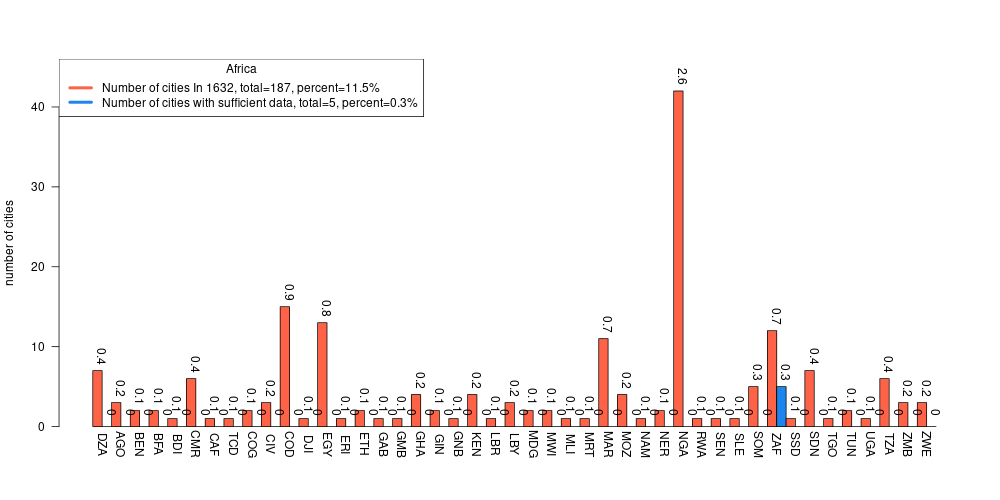
\includegraphics[trim={ 0 35 25 50 },clip,scale=0.45]{Images2/Africa_cities_Rev2.png}
\caption{\bf Number of the largest 1632 global cities in countries and the number of cities after excluding cities with insufficient data in Africa. Text annotations show proportions of total (in percents) for each country.}
 \label{fig:africa}
\end{figure}

\begin{figure}
\centering
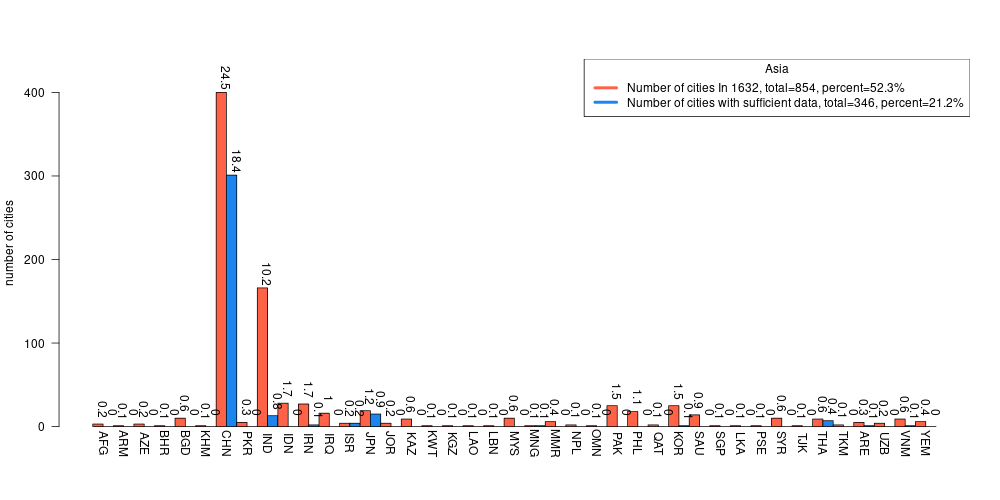
\includegraphics[trim={ 0 35 25 50 },clip,scale=0.45]{Images2/Asia_cities_Rev2.png}
\caption{\bf Number of the largest 1632 global cities in countries and the number of cities after excluding cities with insufficient data in Asia. Text annotations show proportions of total (in percents) for each country.}
 \label{fig:asia}
\end{figure}

\begin{figure}
\centering
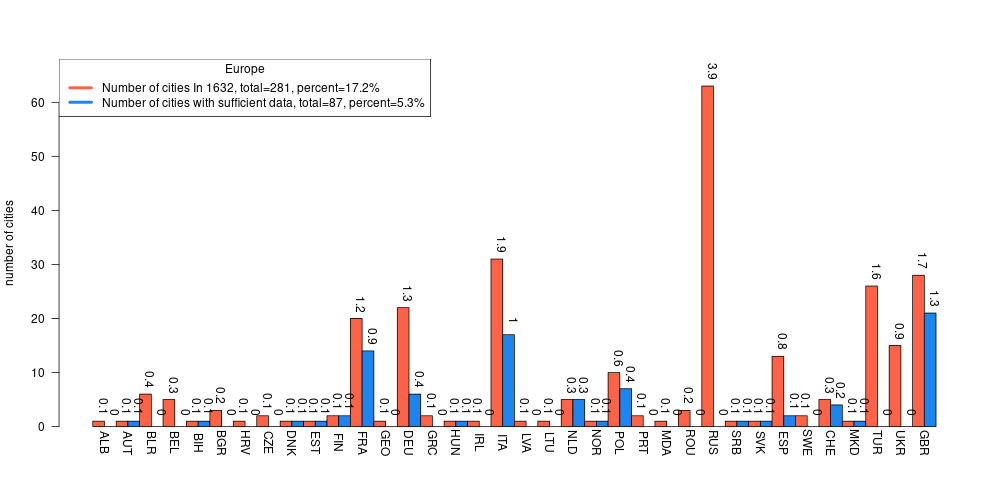
\includegraphics[trim={ 0 35 25 50 },clip,scale=0.45]{Images2/Europe_cities_Rev2.png}
\caption{\bf Number of the largest 1632 global cities in countries and the number of cities after excluding cities with insufficient data in Europe. Text annotations show proportions of total (in percents) for each country.}
 \label{fig:europe}
\end{figure}

\begin{figure}
\centering
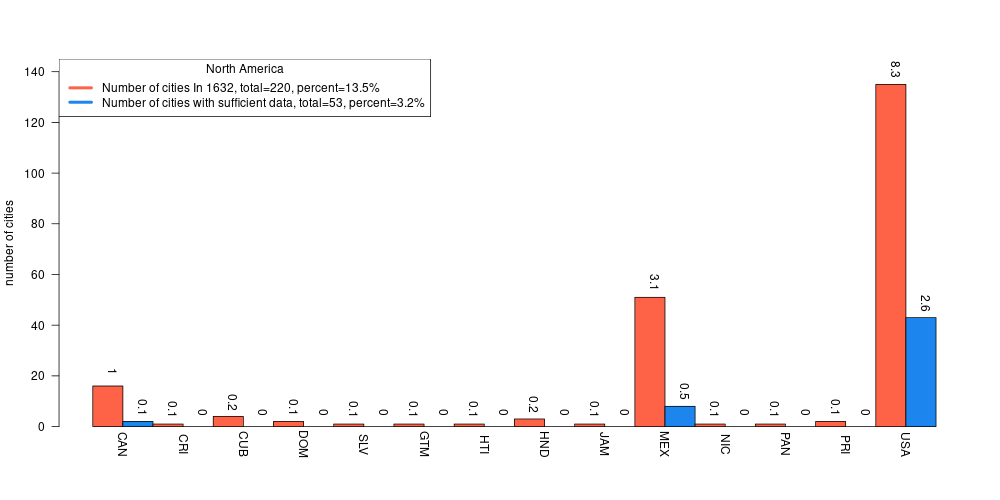
\includegraphics[trim={ 0 35 25 50 },clip,scale=0.45]{Images2/North America_cities_Rev2.png}
\caption{\bf Number of the largest 1632 global cities in countries and the number of cities after excluding cities with insufficient data in North America. Text annotations show proportions of total (in percents) for each country.}
 \label{fig:northamerica}
\end{figure}

\begin{figure}
\centering
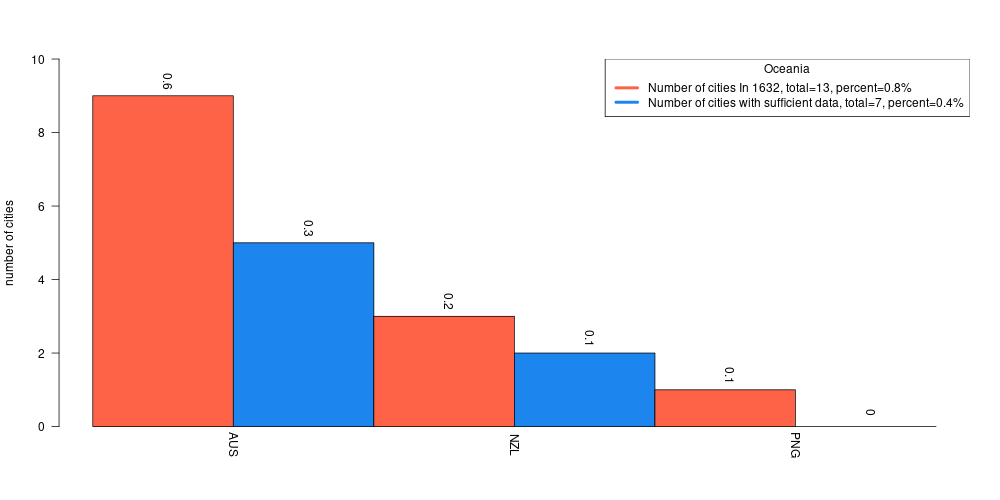
\includegraphics[trim={ 0 35 25 50 },clip,scale=0.45]{Images2/Oceania_cities_Rev2.png}
\caption{\bf Number of the largest 1632 global cities in countries and the number of cities after excluding cities with insufficient data in Oceania. Text annotations show proportions of total (in percents) for each country.}
 \label{fig:oceania}
\end{figure}

\begin{figure}
\centering
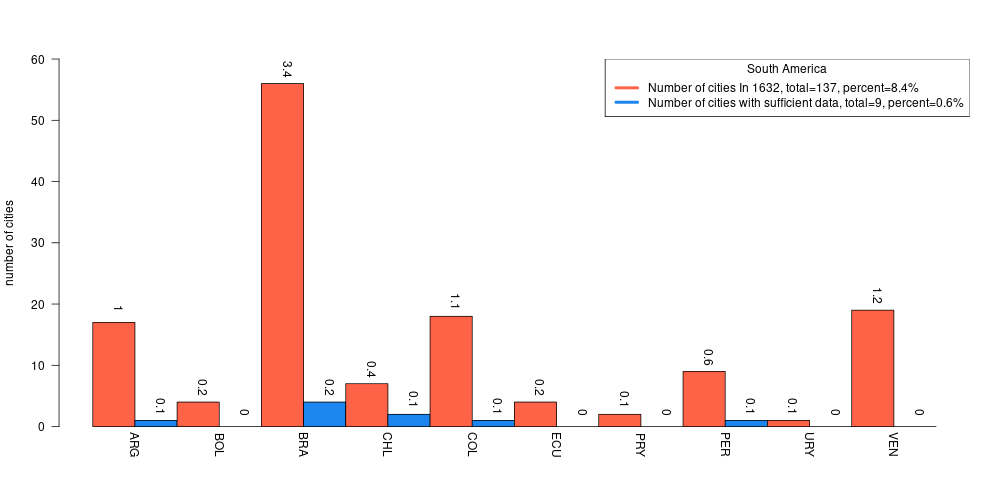
\includegraphics[trim={ 0 35 25 50 },clip,scale=0.45]{Images2/South America_cities_Rev2.png}
\caption{\bf Number of the largest 1632 global cities in countries and the number of cities after excluding cities with insufficient data in South America. Text annotations show proportions of total (in percents) for each country.}
 \label{fig:southhamerica}
\end{figure}


\end{document}
\endinput
%%
%% End of file `elsarticle-template-num.tex'.

